\documentclass[UTF8]{ctexart}
\usepackage{hyperref}
\usepackage{abstract}
\usepackage[margin=1in]{geometry}
\usepackage{graphicx}
\usepackage{gensymb}
\usepackage{amsmath}
\usepackage{float}
\usepackage{ctex,amsmath,amssymb,bm,indentfirst,hyperref,graphicx}
\usepackage{multirow}
\usepackage{cases}
\begin{document}
\title{电磁波在同轴电缆传输线中的传输特性}
\author{2019012137  工物90  张鸿琳}
\maketitle
\begin{abstract}
本实验通过信号发生器产生特定信号,利用示波器观察现象,探究了同轴电缆的一些基本性质。实验中,通过将同轴电缆末端开路和短接测量了同轴电缆的等效电容、等效电感、特征阻抗,同时观测了在不同阻抗交界处信号的反射现象,并由此验证了同轴电缆的特征阻抗大小,并且进一步探究了同轴电缆中的反射波与入射波叠加形成的驻波现象。

\centering
\textbf{Keywords:}信号发生器,示波器,同轴电缆,特征阻抗,驻波
\end{abstract}

\section{实验原理}
\subsection{同轴电缆传输线的等效电容与等效电感}
\paragraph{等效电容}
同轴电缆由同轴的半径为a的导体和半径为b的导体壳组成,二者中间充满相对介电常数为$\epsilon_r$以及相对磁导率为$\mu_r$的介质,设中心导体单位长度电荷量为Q,中心导体与外层导体之间的电势为$U=\int_{a}^{b}Edr=\int_{a}^{b}\frac{Q}{2\pi\varepsilon_0\varepsilon_rr}dr=\frac{Q}{2\pi\varepsilon_0\varepsilon_r}\ln\frac{b}{a}$,故而同轴电缆的单位长度电容为:
\begin{equation}
C=\frac{Q}{U}=\frac{2\pi\varepsilon_0\varepsilon_r}{\ln\frac{b}{a}}
\end{equation}
\paragraph{等效电感}
设电流大小为I,单位长度的同轴电缆的横截面的磁通量$\Phi=\int_{a}^{b}Bdr=\int_{a}^{b}\frac{\mu_0\mu_rI}{2\pi r}dr=\frac{\mu_0\mu_rI}{2\pi}\ln\frac{b}{a}$,则同轴电缆单位长度的电感为:
\begin{equation}
L=\frac{\Phi}{I}=\frac{\mu_0\mu_r}{2\pi}\ln\frac{b}{a}
\end{equation}
\subsection{同轴电缆传输线的特征阻抗}
由上面的分析中求得的等效电感和等效电容,知传输线可以看作等效电感和等效电容的叠加,设单位长度传输线的电阻、电感、电容、电导分别为$R$、$L$、$C$、$G$,$v$为沿传输线方向的电压,$i$为沿传输线方向的电流,设电压电流为简谐变化的,角频率为$\omega$。考虑一小段长度为$\Delta z$的传输线,则有
\begin{equation}
{\lim_{\Delta z \to 0}}\frac{\Delta v}{\Delta z}=\frac{\partial v}{\partial z}=-i(R+j\omega L)
\end{equation}
\begin{equation}
{\lim_{\Delta z \to 0}}\frac{\Delta i}{\Delta z}=\frac{\partial i}{\partial z}=-v(G+j\omega C)
\end{equation}

设传输线传播常数$\gamma$与特征阻抗$Z_0$分别为:
\begin{equation}
\gamma=\sqrt{(R+j\omega L)(G+j\omega C)}=\alpha+j\beta
\end{equation}
\begin{equation}
Z_0=\sqrt{\frac{R+j\omega L}{G+j\omega C}}
\end{equation}

代入公式(3)、(4)中,得到二者满足相同形式的微分方程:
\begin{equation}
\frac{\partial^2y}{\partial z^2}-\gamma^2y=0
\end{equation}

进而得到$v$与$i$的通解为:
\begin{equation}
v=V^+e^{-\gamma z}+V^-e^{\gamma z}=V^+(z)+V^-(z)
\end{equation}
\begin{equation}
i=\frac{1}{Z_0}(V^+e^{-\gamma z}-V^-e^{\gamma z})=I^+(z)+I^-(z)
\end{equation}

那么特征阻抗$Z_0$为:
\begin{equation}
Z_0=\frac{V^+(z)}{I^+(z)}=-\frac{V^-(z)}{I^-(z)}
\end{equation}

当传输线损耗很小时,即$R\ll\omega L$、$G\ll\omega C$时,可证明,$Z_0\approx\sqrt{\frac{L}{C}}$,$\gamma\approx\alpha+j\omega\sqrt{LC}$。
\subsection{脉冲信号在同轴电缆传输线中的传输与反射}
若两根特征阻抗分别为$Z_0$与$Z_1$的传输线连接在一起,且二者之间的连接很短,当振动幅度为$V_i$的信号到达而二者临界面,一部分透射,振幅为$V_t$,一部分被反射,幅度为$V_r$。由两根传输线在临界面处电压幅度一致,有$V_i+V_r=V_t$,同时再由电流在界面处守恒,得到$\frac{V_i}{Z_0}-\frac{V_r}{Z_0}=\frac{V_t}{Z_1}$,解得界面处反射系数为:
\begin{equation}
\Gamma=\frac{V_r}{V_i}=\frac{Z_1-Z_0}{Z_1+Z_0}
\end{equation}


\section{实验仪器及实验步骤}
\subsection{实验仪器}
\noindent
(1). 信号发生器: 用于产生所需的电压信号。\\
(2). 示波器: 记录电路中某一区间的电压变化。\\
(3). 电阻板:提供一系列电阻。\\
(4). BNC三通接头、BNC转香蕉头线、BNC-BNC短测试线:用于电路连接。\\
(5). 待测BNC-BNC同轴电缆
\subsection{实验步骤}
\subsubsection{测试待测同轴电缆的等效电容和等效电感}
设置信号发生器,使之输出电压峰值为10Vpp,初始频率$f$为60kHz,输出阻抗为50$\Omega$的正弦信号。将同轴电缆的一端与一个1000$\Omega$的电阻作为标准电阻$R$串联,另一端开路,信号发生器作为电源,使用示波器的CH1通道测量总电压$V_A$,CH2测量同轴电缆两端电压。微调信号发生器输出频率,使$V_C$约为$V_A$的$\frac{1}{\sqrt{2}}$,记录$f$、$V_A$和$V_C$的值。

\textbf{为了满足信号发生器与示波器的两个通道的“共地”要求},即三者的测试线负极需要接在一起,需要交换标准电阻$R$和同轴电缆的位置,重新连接电路,CH2改为测量电阻两端电压,由此得到$V_R$。

测量同轴电缆的电感时,将信号发生器的初始频率$f$设为300kHz,标准电阻更换为30$\Omega$,同时在同轴电缆末端接上一根BNC转香蕉头线,将其短路,之后测量过程与测量等效电容的过程一致,得到$f'$、$V_A'$、$V_L$和$V_R'$。

\subsubsection{脉冲信号在同轴电缆中的传输与反射,并由此计算特征阻抗}
将信号发生器波形设置为脉冲,频率为40kHz,幅度为10Vpp,占空比为0.2$\%$。电路中串联两个1$k\Omega$的电阻,将同轴电缆一端与靠近信号发生器负极的电阻并联,另一端开路,使用示波器的CH1测量同轴电缆起始端的信号,CH2测量同轴电缆末端的信号,记录各个波形的幅度和相对起始脉冲的延时。再将示波器CH2的测试线移动至第5段和第6段电缆之间,观测此处的入射波和反射波信号。

再将同轴电缆末端短路,重复上述实验过程。

使用装有$10\Omega$串联电阻的电阻板作为负载电阻,反复调节接入的阻值大小,直到反射信号最小,则此时负载电阻值约等于传输线特征阻抗。
\subsubsection{简谐信号在同轴电缆传输线中的驻波}
计算出传输线中形成驻波所需的频率,设置信号发生器输出为正弦波形,电压峰值设为10Vpp,设置频率为计算所得的频率,使用示波器测量同轴电缆起始端、中点处、末端的电压波形,观察现象。

\section{数据处理}
\subsection{测试待测同轴电缆的等效电容和等效电感的相关数据的处理}
同轴电缆末端开路时,有如下数据
    \begin{table}[H]
\centering
    \caption{测量等效电容所得数据}  
    \begin{tabular}{|c|c|c|c|}
    \hline  
    $V_A$(V) & $V_C$(V)  &$V_R$(V) &$f$(kHz) \\  
    \hline  
    10.24  & 7.3 & 6.5&60 \\  
    \hline  
    \end{tabular}  
    \end{table}  

故而$Z_C=\frac{7.3}{6.5}\times1000\approx1123\Omega$,$C_{total}=\frac{1}{2\pi fZ_C}\approx2.362\times10^{-9}$F,进而得到$C=\frac{C_{total}}{l}\approx7.87\times10^{-11}$F/m。

同轴电缆短路时,有如下数据
    \begin{table}[H]
\centering
    \caption{测量等效电感所得数据}  
    \begin{tabular}{|c|c|c|c|}
    \hline  
    $V_A'$(V) & $V_L$(V)  &$V_R'$(V) &$f'$(kHz) \\  
    \hline  
    5.62  & 3.92 & 3.52 & 390 \\  
    \hline  
    \end{tabular}  
    \end{table} 

故而$Z_L=\frac{V_L}{V_R'}R'\approx33.4\Omega$,$L_{total}=\frac{Z_L}{2\pi f'}\approx1.36\times10^{-5}$H,进而得到$L=\frac{L_{total}}{l}\approx4.54\times10^{-7}$H/m。

同轴电缆横截面上的电力线和磁力线分布示意图如下
\begin{figure}[H]
\centering
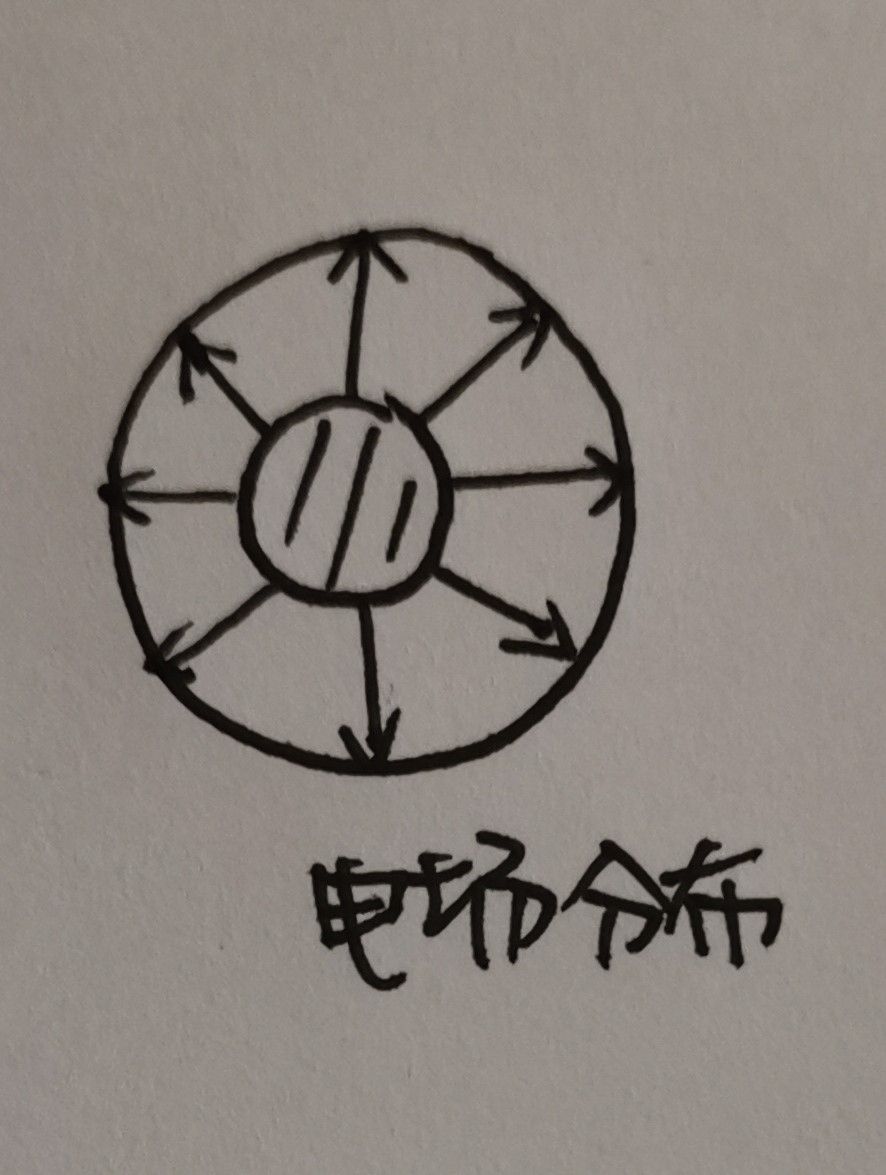
\includegraphics[width=0.35\textwidth]{AA.jpg}
\caption{电场分布示意图}
\end{figure}
\begin{figure}[H]
\centering
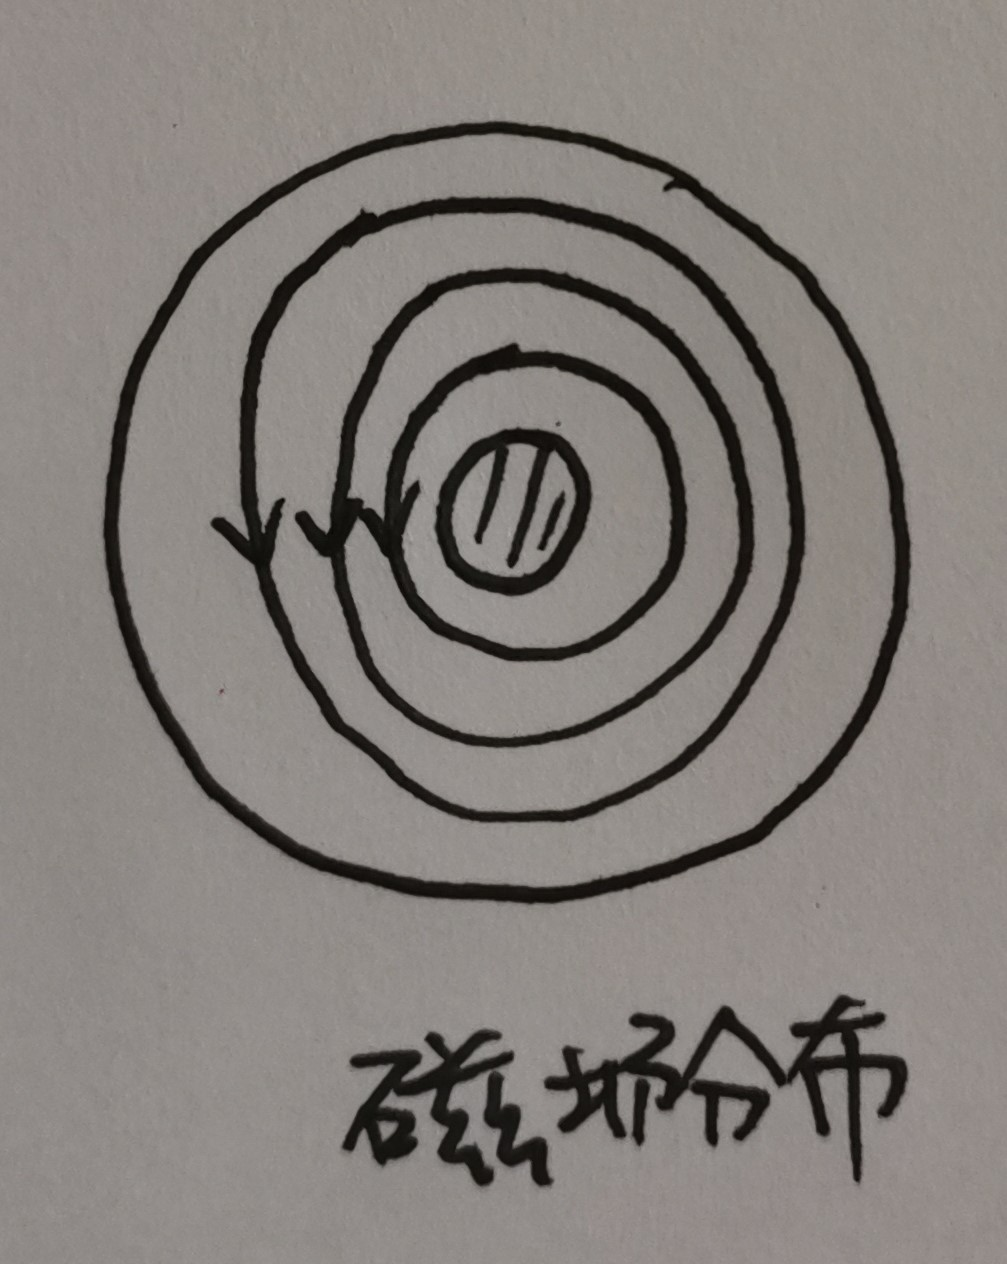
\includegraphics[width=0.35\textwidth]{BB.jpg}
\caption{磁场分布示意图}
\end{figure}
趋肤电流分布在中心导体外表面以及外层导体内表面一侧。

再利用上述数据,由实验原理中关于特征阻抗的分析,可计算出该同轴电缆的特征阻抗为$Z_0\approx \sqrt{\frac{L}{C}}\approx75.95\Omega$,同时可得电磁波在同轴电缆中传播的相速度为$v_p=\frac{1}{\sqrt{LC}}\approx1.67\times10^8$m/s,截止相对介电常数为$\varepsilon_r=(\frac{c}{v_p})^2\approx3.22$。

假设实验中测试的同轴电缆是一根半无限长的同轴电缆传输线且无损耗($R=G=0$),信号发生器发出电压峰值为10Vpp,频率为50kHz的正弦信号,虽然是半无限长电缆,但是根据特征阻抗定义,半无限长同轴电缆的特征阻抗仍为$Z_0$,故而半无限长同轴电缆向外输送功率,且输出功率为$P_{out}=\frac{U^2}{2Z_0}=\frac{100}{2\times75.95}\approx$0.6583W,能量储存在同轴电缆中生成的电磁波中,或者说存储在同轴电缆的等效电容和等效电感中。
\subsection{脉冲信号在同轴电缆传输线中的传输与反射}
由实验原理中的分析,得到反射系数$\Gamma=\frac{V_r}{V_i}=\frac{Z_1-Z_0}{Z_1+Z_0}$,故而可知:
\begin{itemize}
\item 当$Z_0=Z_1$时,即在阻抗匹配条件下,在界面处信号不会发生反射
\item 当$Z_1<Z_0$时,反射信号与入射信号相位变化为$\pi$
\end{itemize}

相应地进行了如下情况的实验:
\begin{itemize}
\item 当末端开路时,即$Z_L=\infty $时,信号反射后沿-z方向传播
\item 当末端短路时,即$Z_L=0$时,信号反射并反相后沿-z方向传播
\item 当末端接匹配负载时,即$Z_L=Z_0$时,信号没有反射波,只有沿+z方向传播的行波
\end{itemize}

整理原始数据,得到下表
\begin{table}[H]
    \centering
\caption{观测脉冲信号在传输线中传播所得数据}
    \begin{tabular}{|l|l|l|l|l|l|}
    \hline
        同轴电缆末端状态 & \multicolumn{2}{|c|}{信号幅度$V_i$(mV)}   &\multicolumn{2}{|c|}{信号延时$\tau_i$(ns)}   \\ \hline
        \multirow{7}{*}{开路} & $V_0$ & 0.715 & $\tau_0$ & 10.8 \\ \cline{2-5}
         & $V_1$ & 1.13 & $\tau_1$ & 196.8 \\  \cline{2-5}
         & $V_2$ & 0.783 & $\tau_2$ & 378.8 \\  \cline{2-5}
         & $V_3$ & 0.566 & $\tau_3$ & 562.8 \\ \cline{2-5}
         & $V_4$ & 0.421 & $\tau_4$ & 742.8 \\  \cline{2-5}
         & $V_5$ & 0.3125 & $\tau_5$ & 922.8 \\  \cline{2-5}
         & $V_6$ & 0.244 & $\tau_6$ & 1068.8 \\ \hline
        \multirow{7}{*}{短路}  & $V_0'$ & 0.698 & $\tau_0'$ & -390.4 \\ \cline{2-5}
         & $V_1'$ & 0 & $\tau_1'$ &  \\ \cline{2-5}
         & $V_2'$ & -0.82 & $\tau_2'$ & -38.4 \\ \cline{2-5}
         & $V_3'$ & 0 & $\tau_3'$ &  \\\cline{2-5}
         & $V_4'$ & 0.405 & $\tau_4'$ & 313.6 \\\cline{2-5}
         & $V_5'$ & 0 & $\tau_5'$ &  \\ \cline{2-5}
         & $V_6'$ &  & $\tau_6'$ &  \\ \hline
    \end{tabular}
\end{table}

将示波器CH2测试线从同轴电缆末端移至第5段和第6段电缆之间后,z=0处和z=$\frac{5}{6}$l处的信号波形示意图如下:
\begin{figure}[H]
\centering
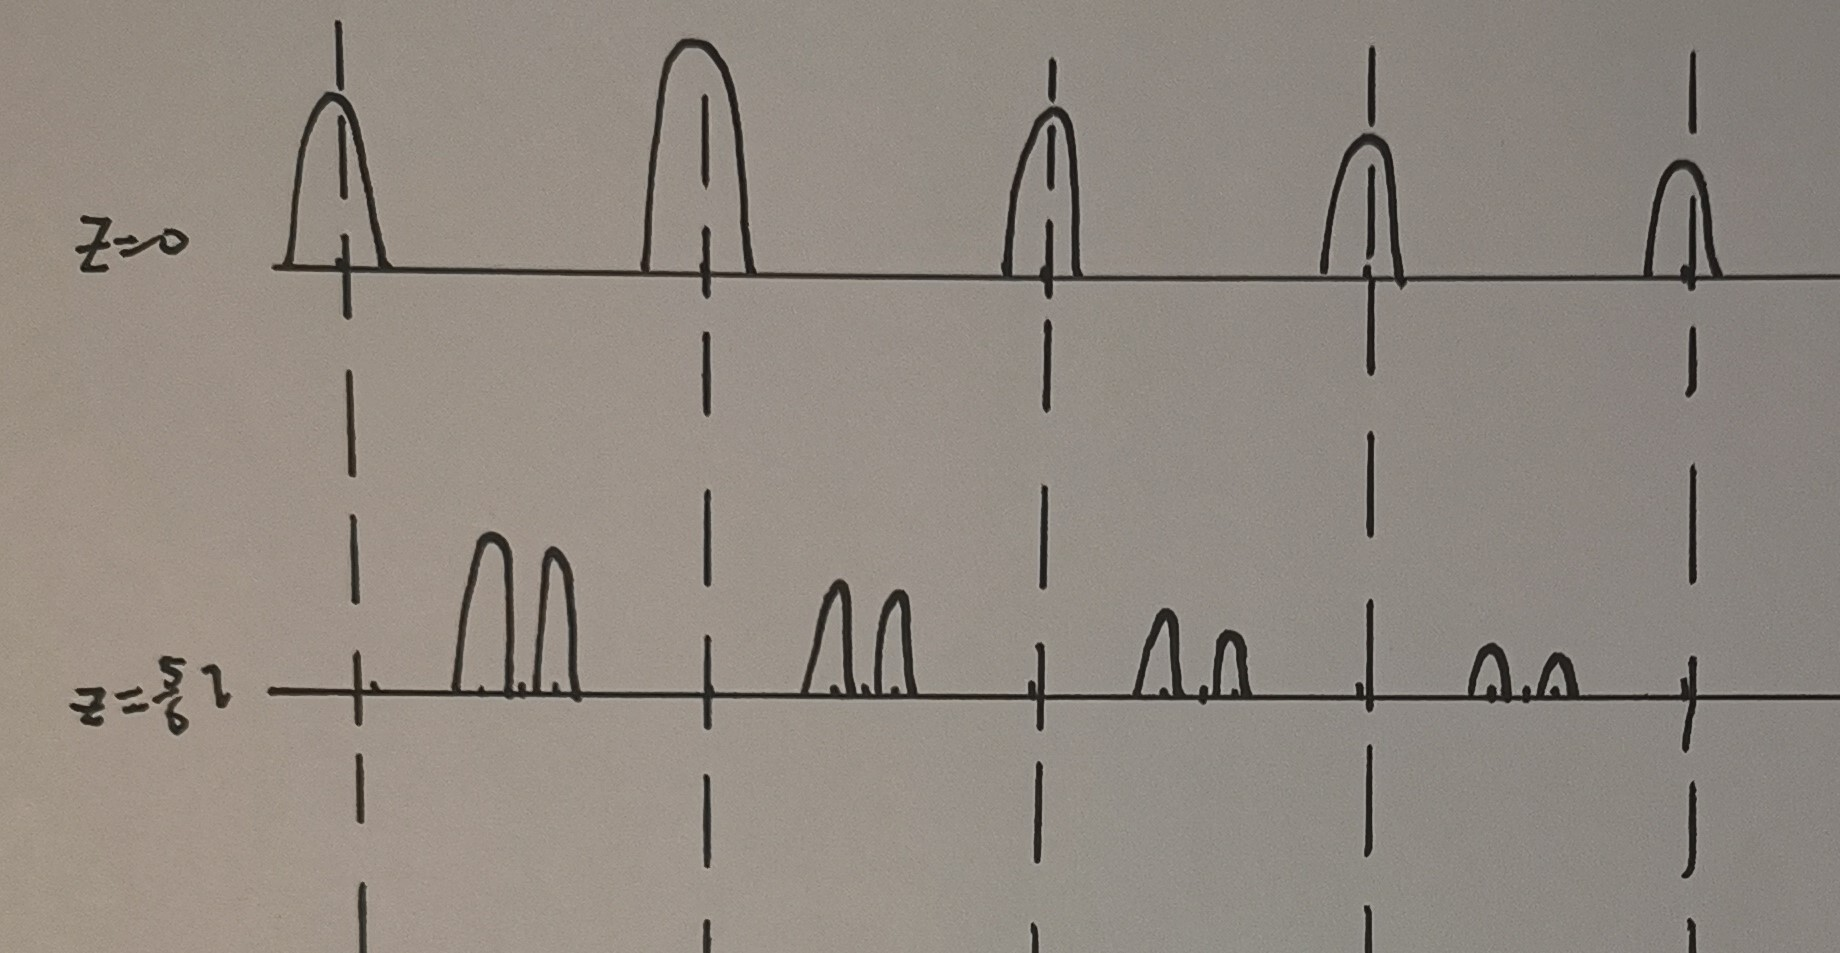
\includegraphics[width=0.95\textwidth]{F.jpg}
\caption{末端开路时信号波形示意图}
\end{figure}

\begin{figure}[H]
\centering
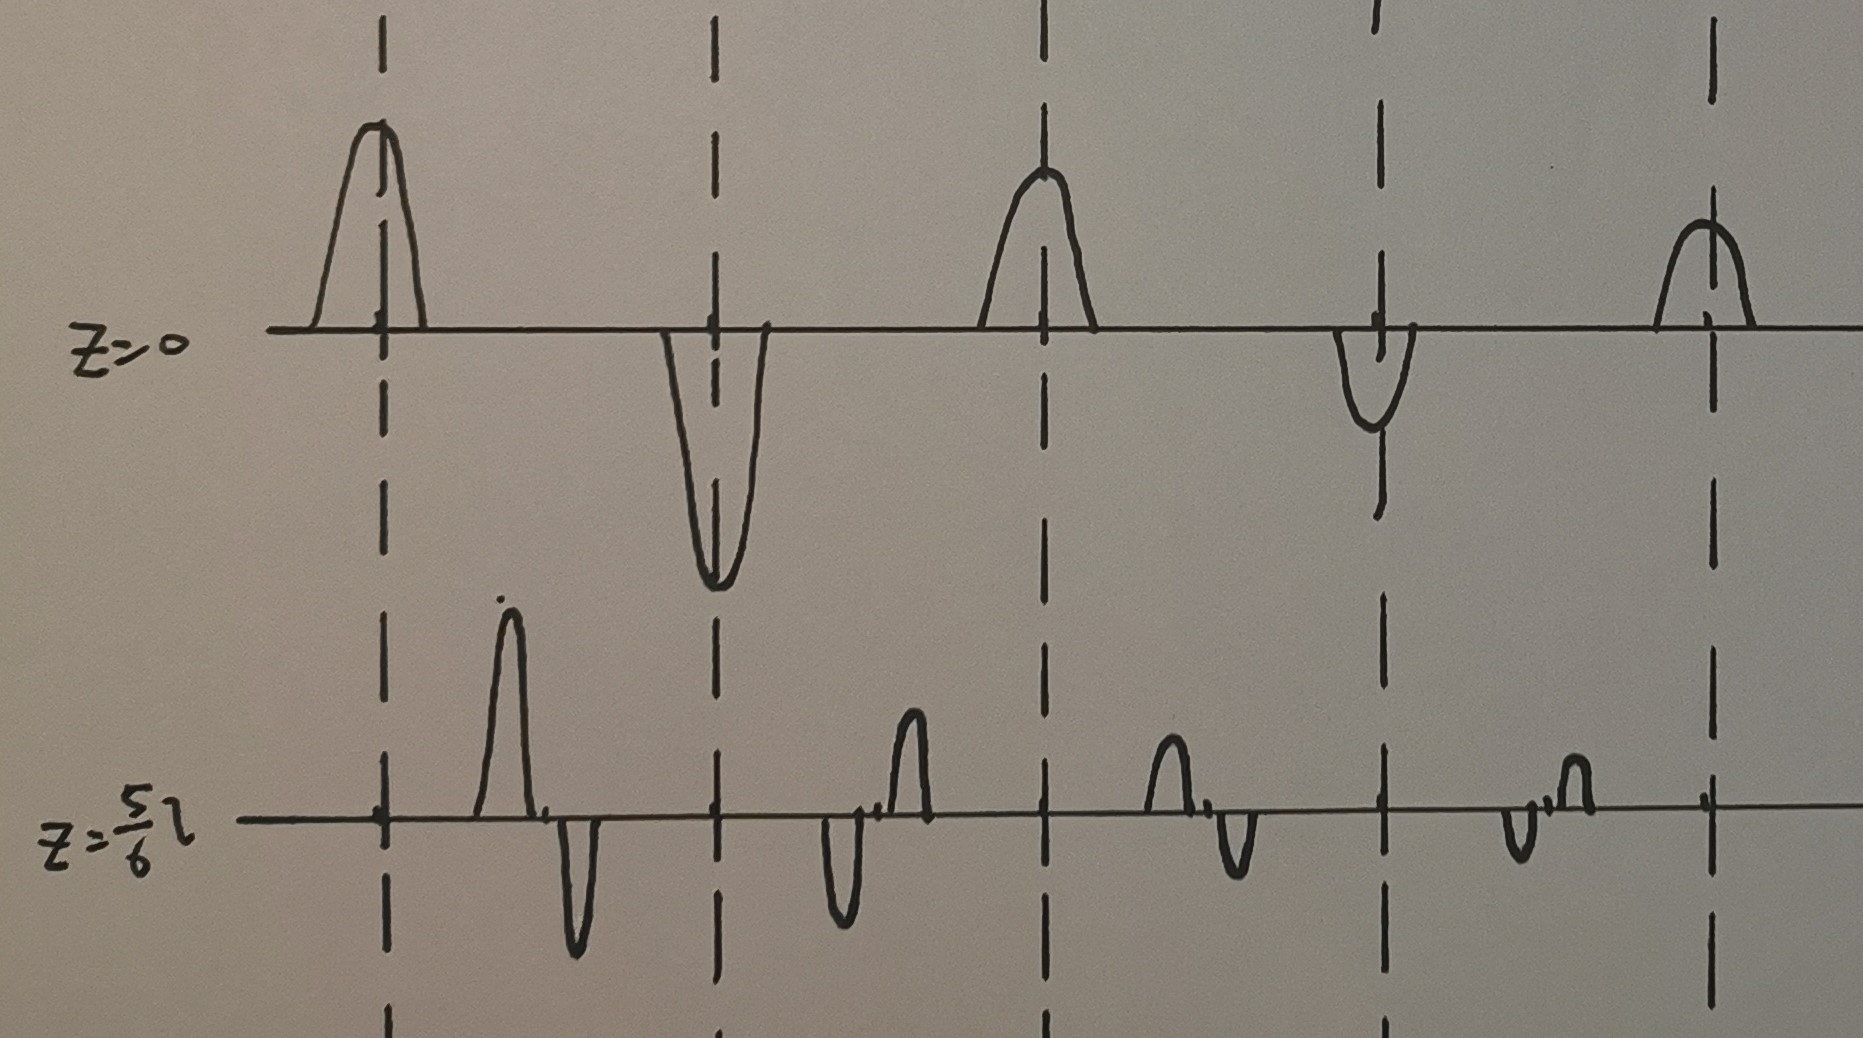
\includegraphics[width=0.95\textwidth]{E.jpg}
\caption{末端短路时信号波形示意图}
\end{figure}


实验中,阻抗匹配条件下的负载电阻约为70$\Omega$到80$\Omega$,与计算所得75.95$\Omega$基本相符。

利用开路时的幅度,$V_1$、$V_2$、$V_3$、$V_4$、$V_5$、$V_6$计算衰减系数$\alpha$,得到$V=V_1'exp(-0.0102l)$($V_1'$为拟合得到的初始电压),即$\alpha\approx0.0102$,拟合程度见下图(其中系列1为实验数据对应曲线,系列2为拟合所得曲线)
\begin{figure}[H]
\centering
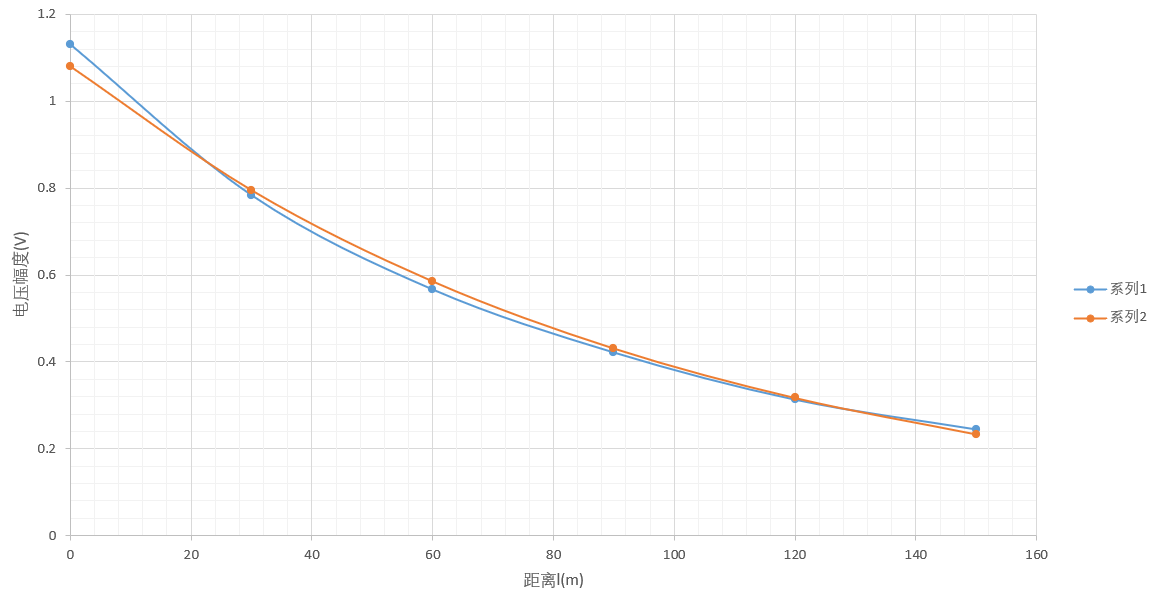
\includegraphics[width=0.95\textwidth]{C.png}
\caption{电压幅度随距离的衰减曲线对比}
\end{figure}

同时,在实验数据中看到,末端开路时$V_1>V_0$,该现象发生的原因是在初始端和末端处发生了入射波和反射波的叠加,所以除$V_0$外其他电压幅度数据应该除以二,才为实际的入射波或者反射波信号幅度。由信号振幅衰减公式,可知经过处理后$\ln(V)$与$l$应为线性关系,实际实验数据处理后得到下图:
\begin{figure}[H]
\centering
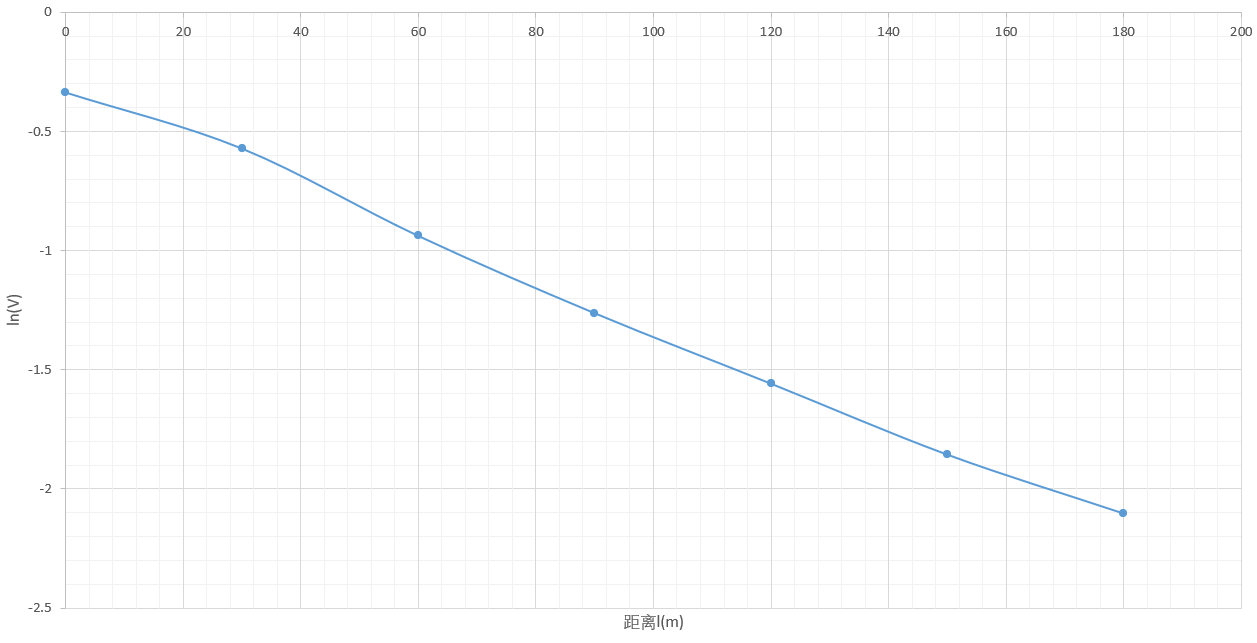
\includegraphics[width=0.95\textwidth]{D.png}
\caption{将除$V_0$外的电压幅度除以2,得到的$\ln(V)$随$l$的变化曲线}
\end{figure}

从图中看出,经过处理后,$\ln(V)$与$l$基本满足线性关系,所以该解释应为合理的。

\subsection{简谐信号在同轴电缆中产生驻波}
当传输线末端开路时,电压反射信号表达式为$V^-(z)=V^-e^{j(\omega t+\beta z+\varphi_1)}$,则总电压表达式如下
\begin{equation}
V=V^+e^{j(\omega t-\beta z+\varphi_0)}+V^-e^{j(\omega t+\beta z+\varphi_1)}
\end{equation}

由于实验中的同轴电缆相当于两端开路,故而,为了形成驻波,要让入射波和反射波都保持稳定,即二者满足两端的边界条件,故而有

\begin{equation}
\left\{
    \begin{array}{l}
            V^+(0)=V^-(0) \\  V^+(l)=V^-(l)
        \end{array}
\right.
\end{equation}

解得$\beta L=k\pi$,而$f=\frac{v_p}{\lambda}=\frac{\beta v_p}{2\pi}$,进而得到$f=\frac{kv_p}{2L}$,此时形成驻波的最低两个频率为$f_1=2783333$Hz、$f_2=5566667$Hz,同轴电缆起始端、中点处、末端的电压波形随时间的变化关系示意图如下:
\begin{figure}[H]
\centering
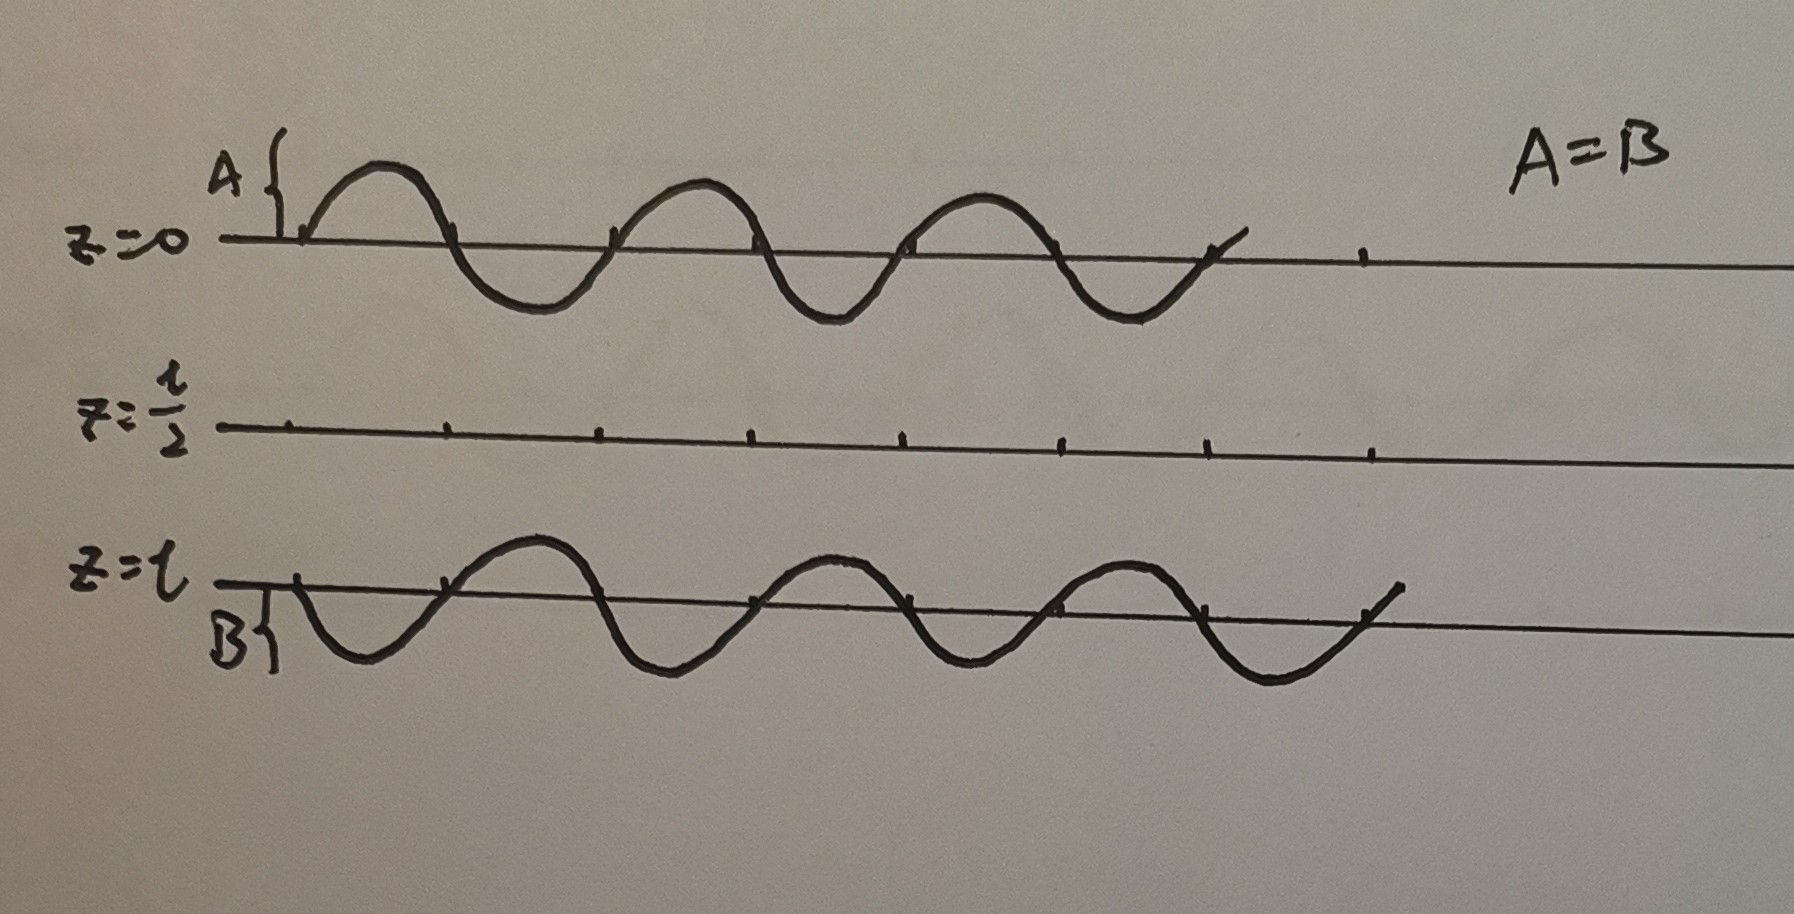
\includegraphics[width=0.95\textwidth]{G.jpg}
\caption{末端开路,$f_1=2783333$Hz时,各处信号示意图}
\end{figure}

\begin{figure}[H]
\centering
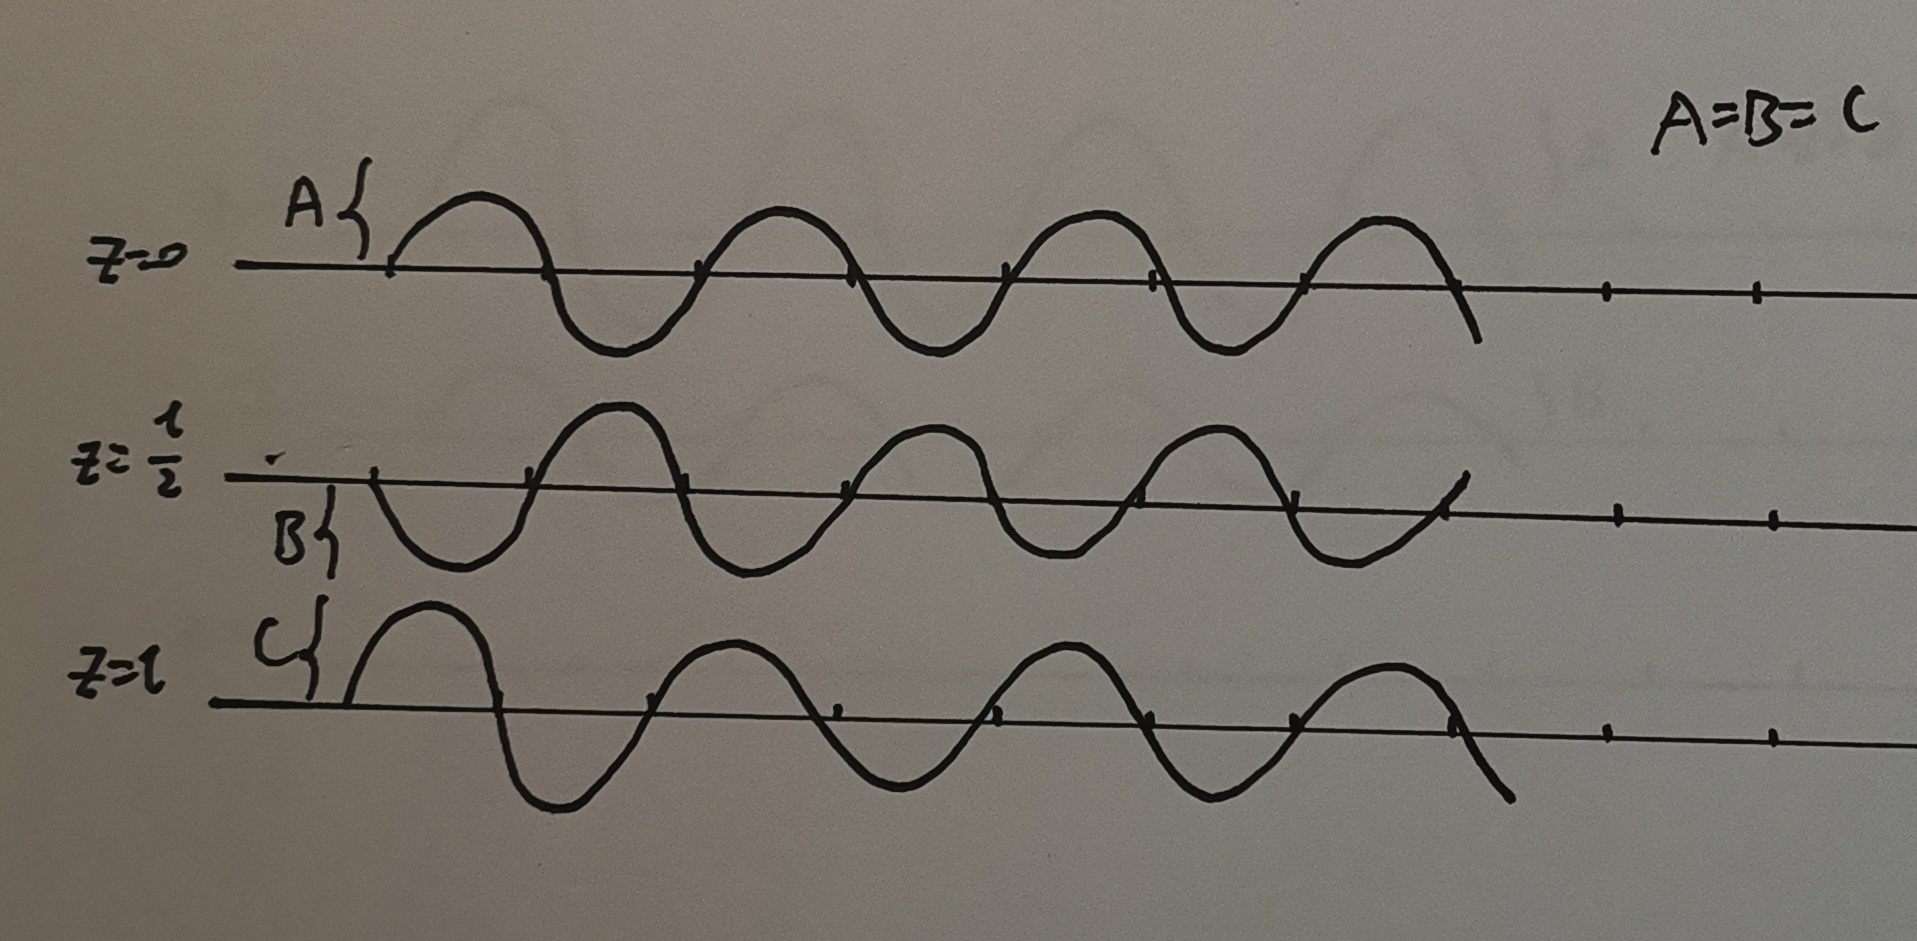
\includegraphics[width=0.95\textwidth]{H.jpg}
\caption{末端开路,$f_2=5566667$Hz时,各处信号示意图}
\end{figure}

在最低两个驻波频率处,沿传输线长度方向的电压信号幅度分布示意图如下:

\begin{figure}[H]
\centering
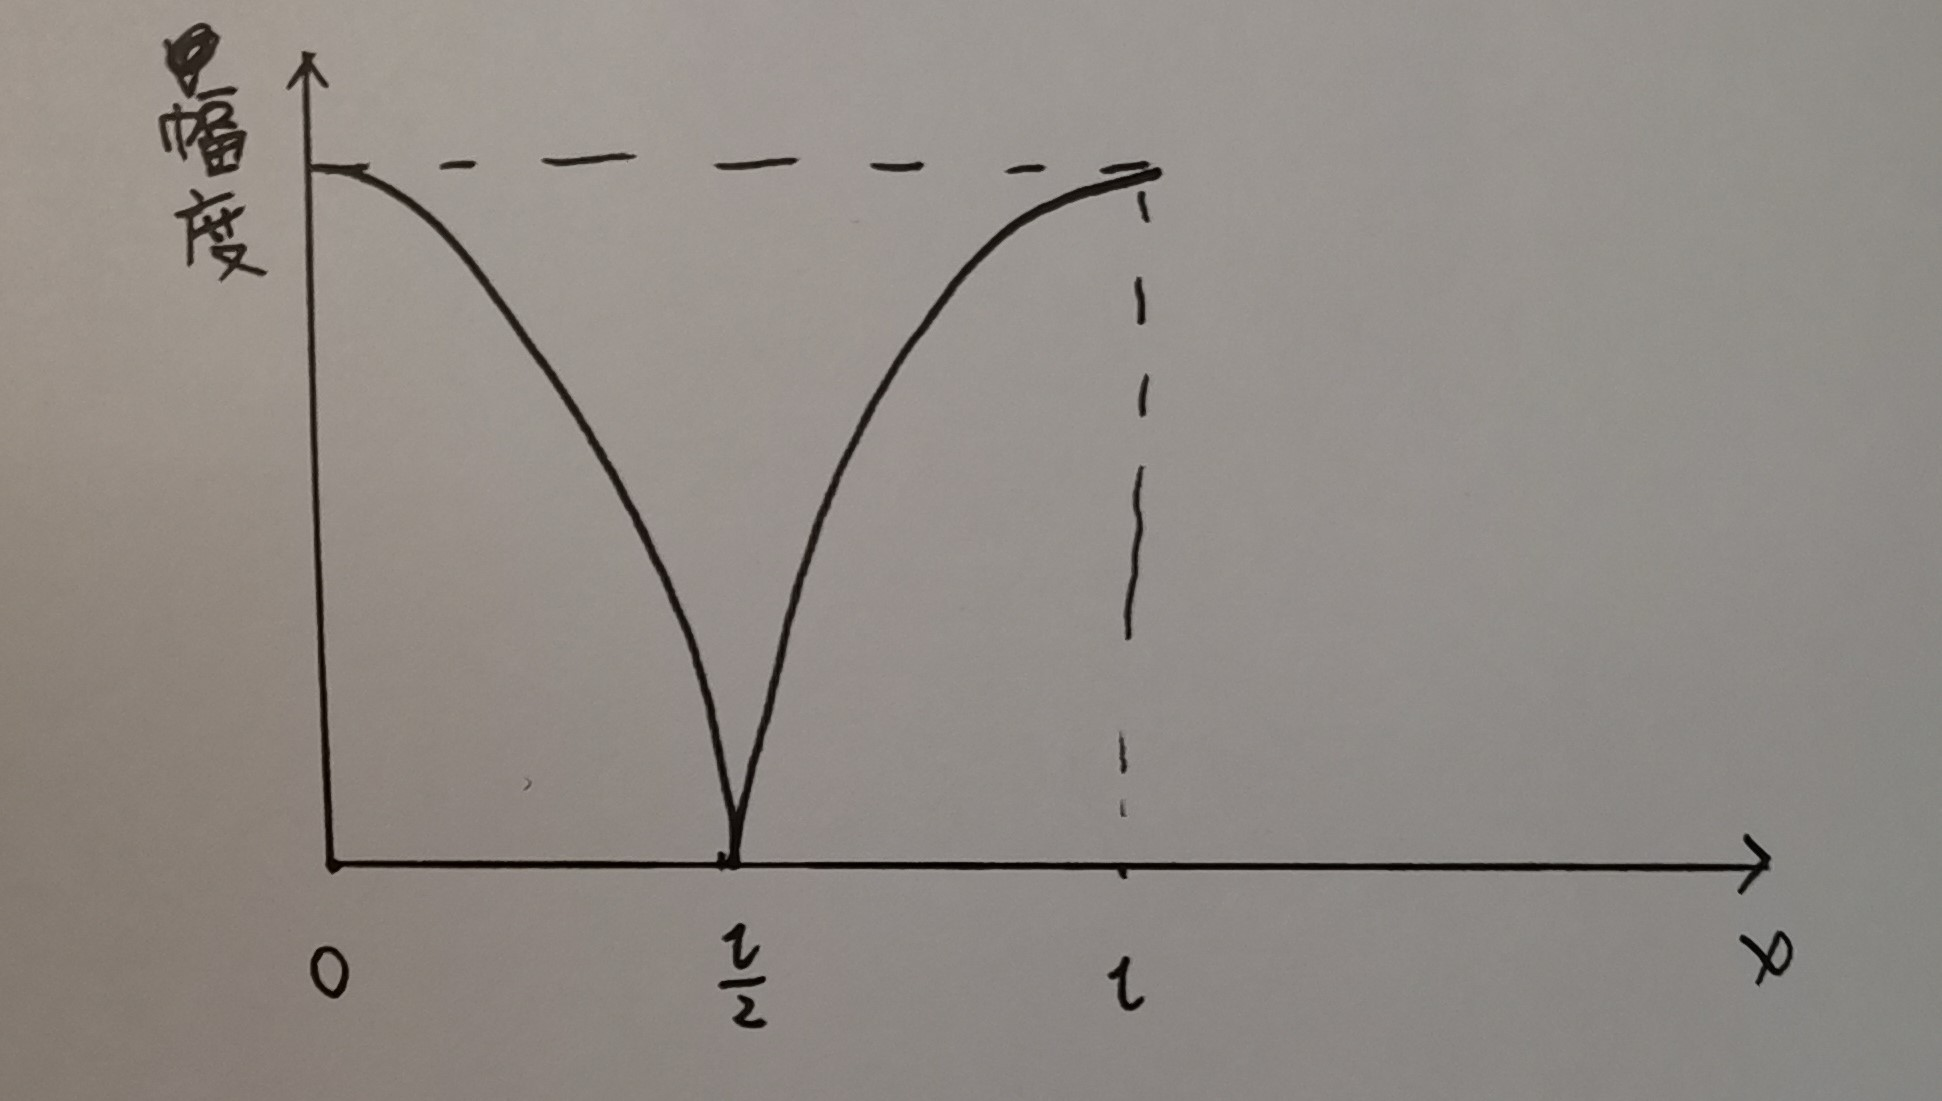
\includegraphics[width=0.95\textwidth]{K.jpg}
\caption{末端开路,$f_1=2783333$Hz时,各处信号幅度}
\end{figure}

\begin{figure}[H]
\centering
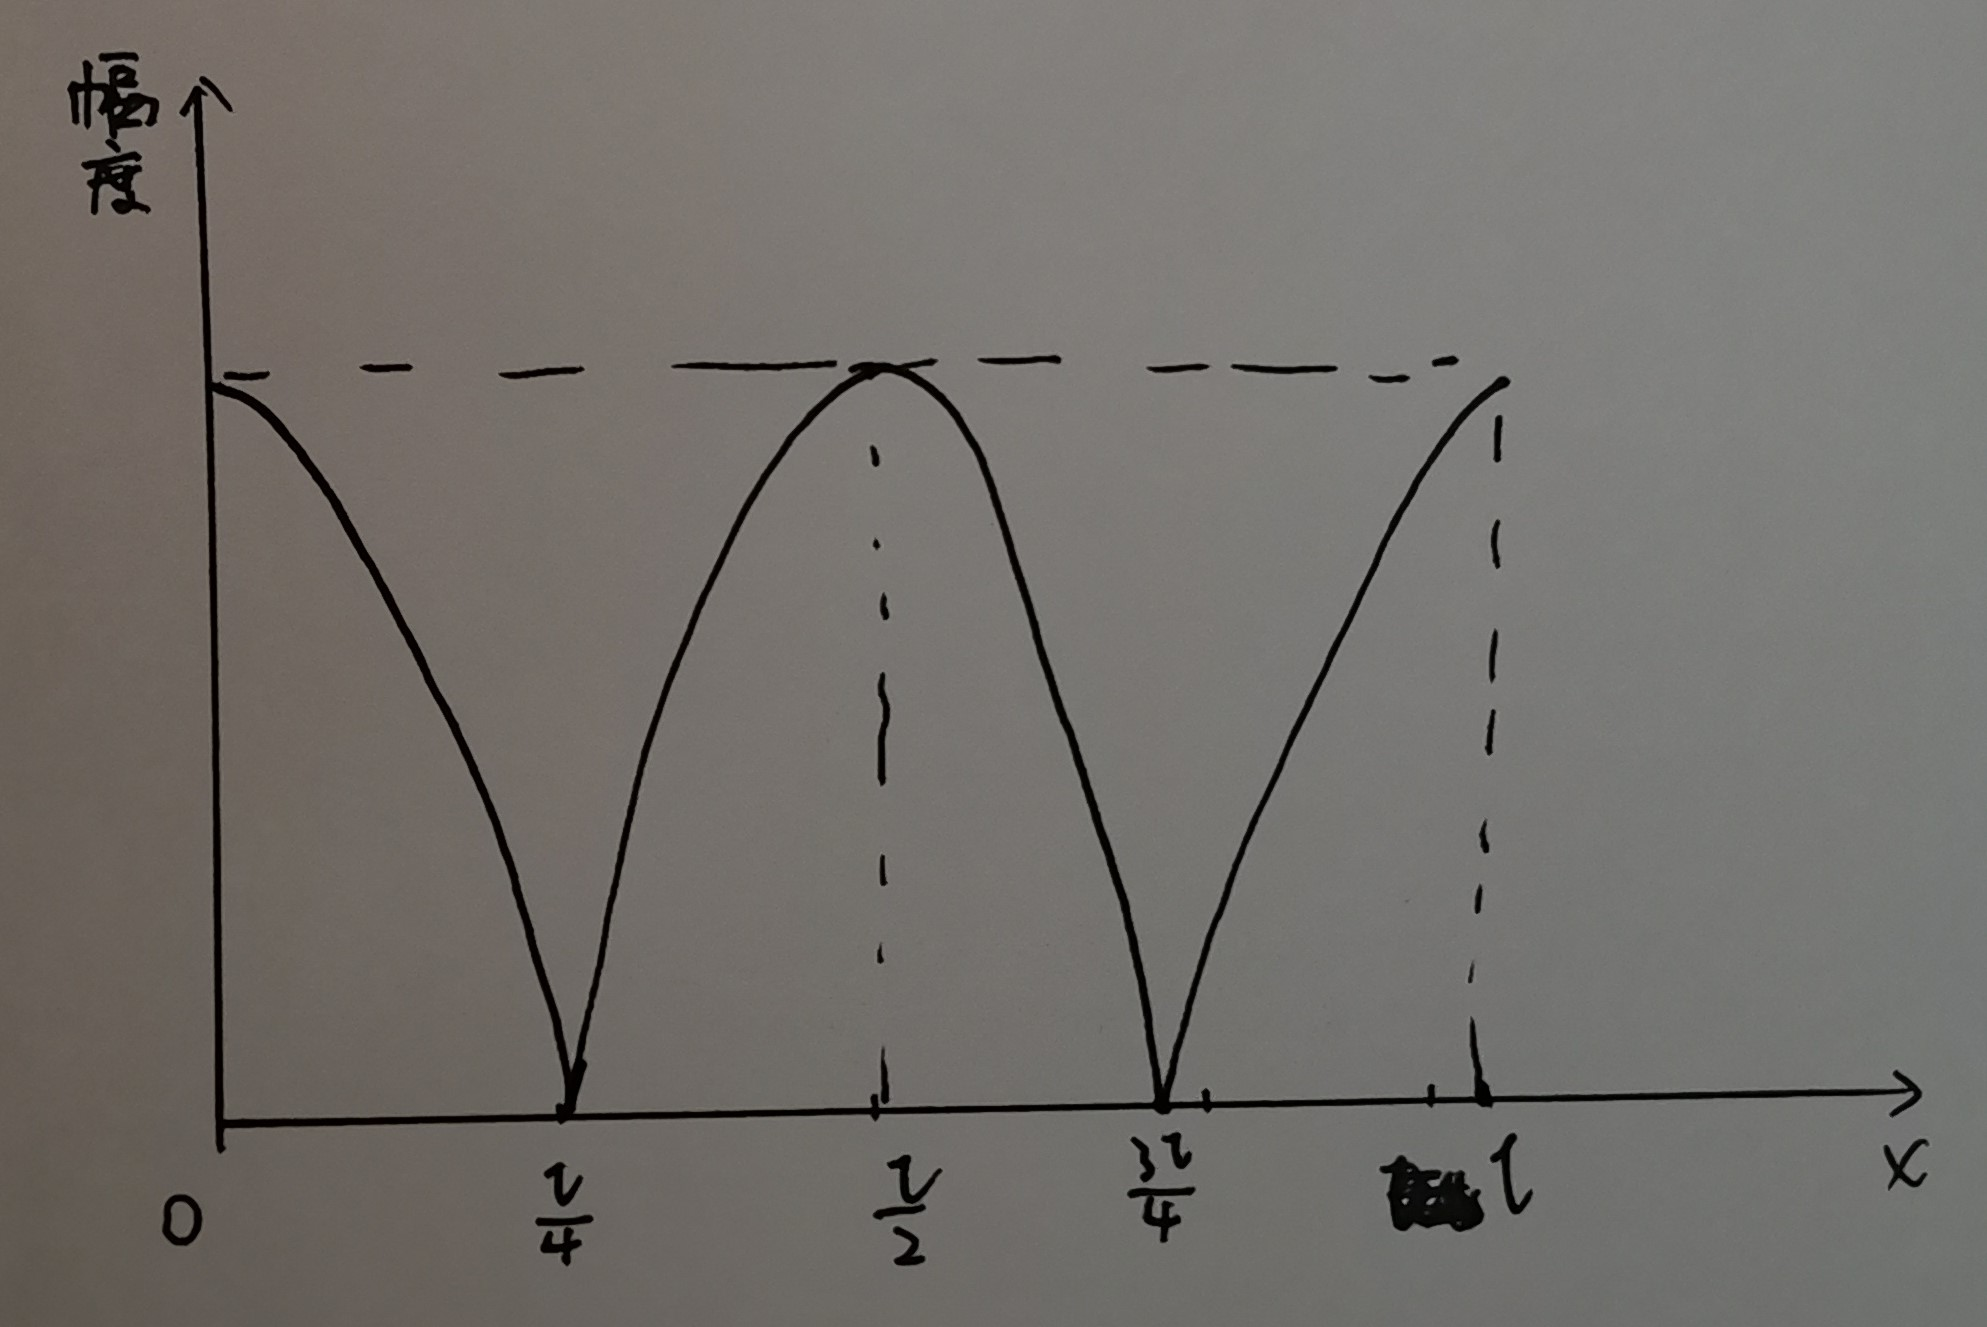
\includegraphics[width=0.95\textwidth]{L.jpg}
\caption{末端开路,$f_2=5566667$Hz时,各处信号幅度}
\end{figure}


开路时,边界处应满足
\begin{equation}
\left\{
    \begin{array}{l}
            V^+(0)=V^-(0) \\  V^+(l)=-V^-(l)
        \end{array}
\right.
\end{equation}

由此得到$f=\frac{(2k+1)v_p}{4L}$,最低两个驻波频率分别为$f_1'=1391666$Hz,$f_2'=4175000$Hz,在满足这两个驻波频率时,同轴电缆起始端、中点处、末端的电压波形随时间的变化关系示意图如下:

\begin{figure}[H]
\centering
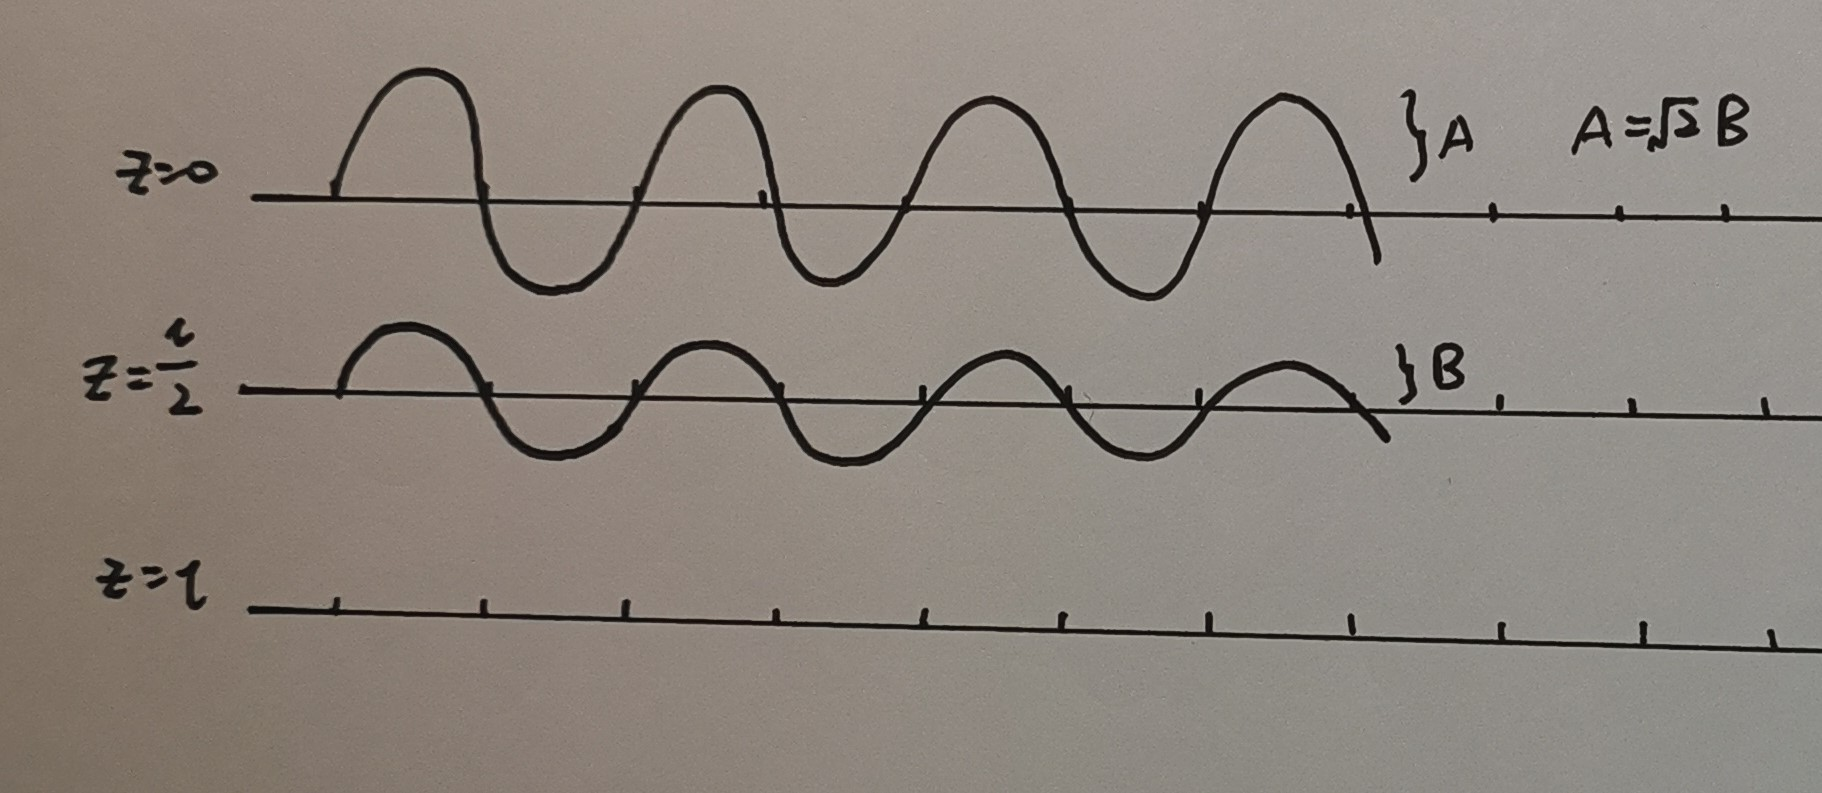
\includegraphics[width=0.95\textwidth]{I.jpg}
\caption{末端短路,$f_1'=1391666$Hz时,各处信号示意图}
\end{figure}

\begin{figure}[H]
\centering
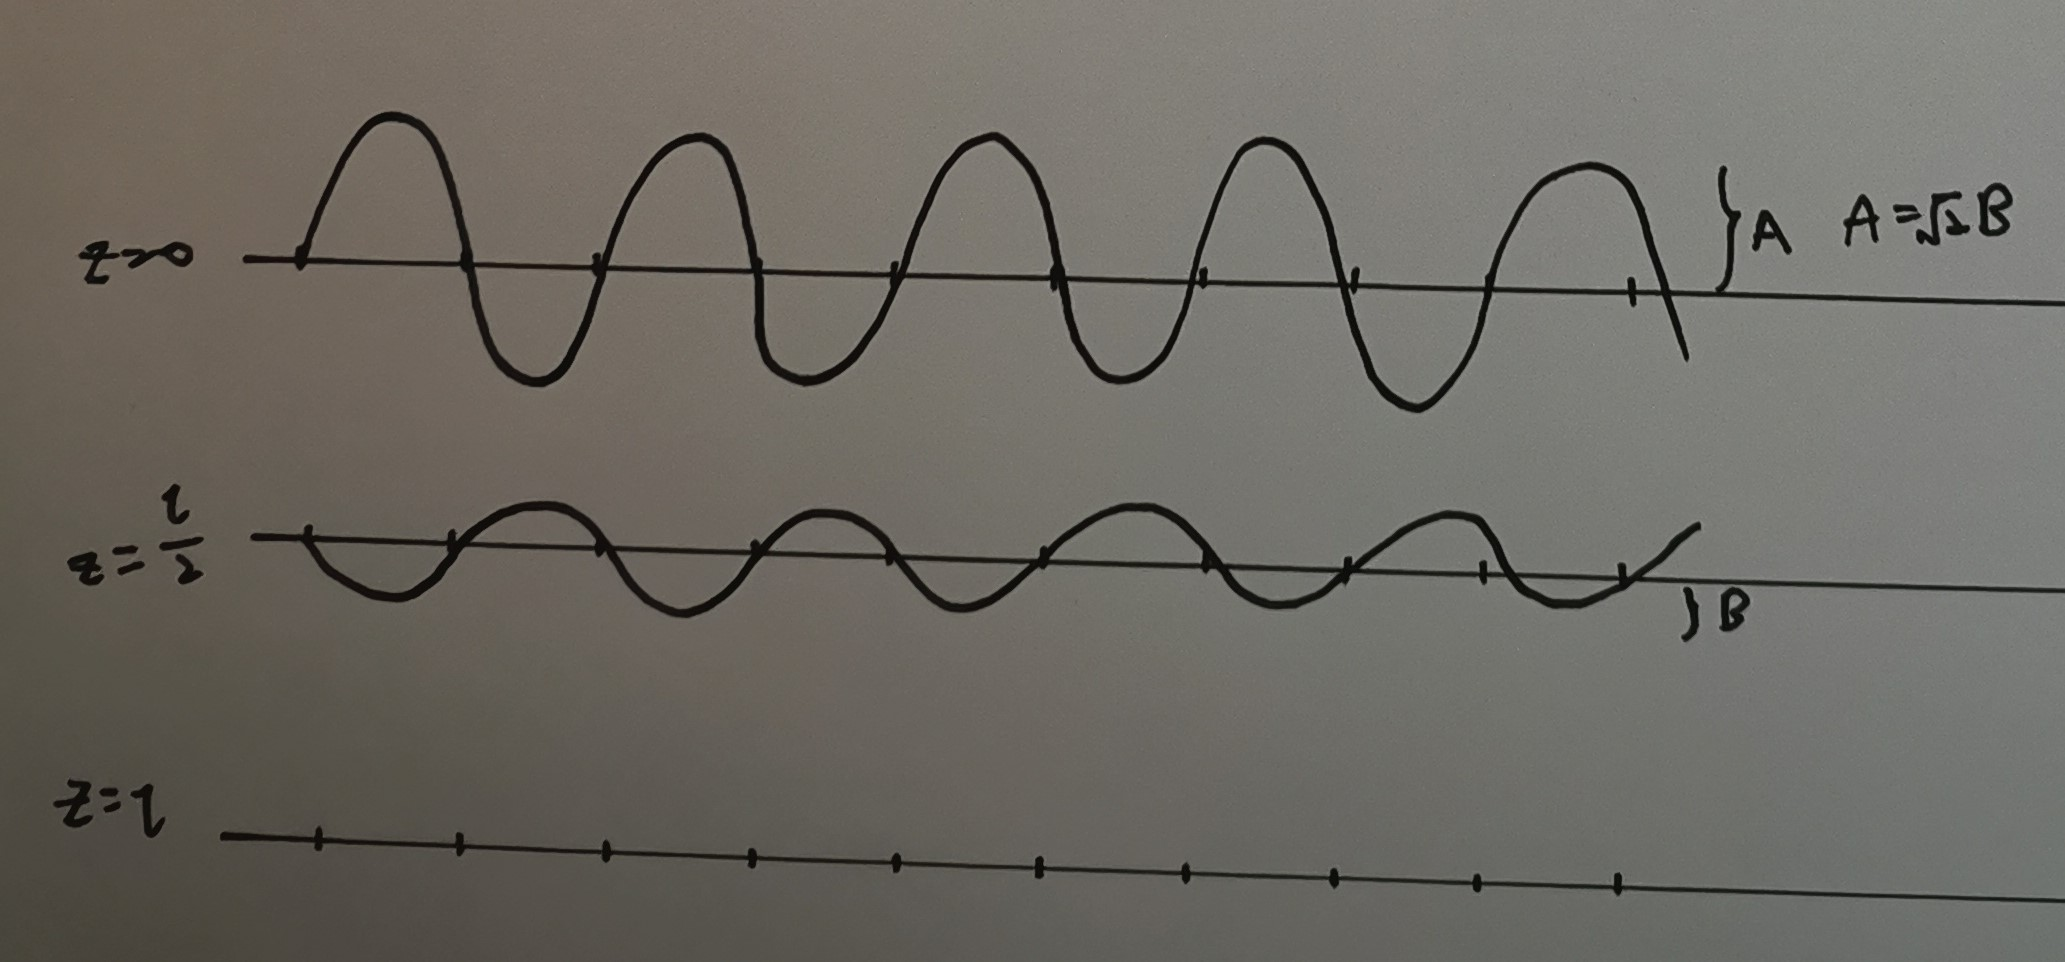
\includegraphics[width=0.95\textwidth]{J.jpg}
\caption{末端短路,$f_2'=4175000$Hz时,各处信号示意图}
\end{figure}

\section{讨论}
这里对实验中存在的一些可能产生误差的因素进行讨论:
\begin{itemize}
\item 在实验时发现,挪动导线和同轴电缆时,示波器上的波形有较大波动和变化,可能是因为弯折造成阻抗等电缆的属性的改变,这可能会造成一定误差
\item 在实验中,由于同轴电缆初始端相当于开路,脉冲信号会在电路中反复反射,在脉冲发出时,上一个脉冲的影响可能还未完全消耗殆尽,这可能会对测得的电压幅度有些影响
\item 实验中的同轴电缆由多段电缆连接组成,各个连接处的接触电阻可能会对实验结果产生影响
\end{itemize}
\section{原始测量数据}
原始测量数据见下图:
\begin{figure}[H]
\centering
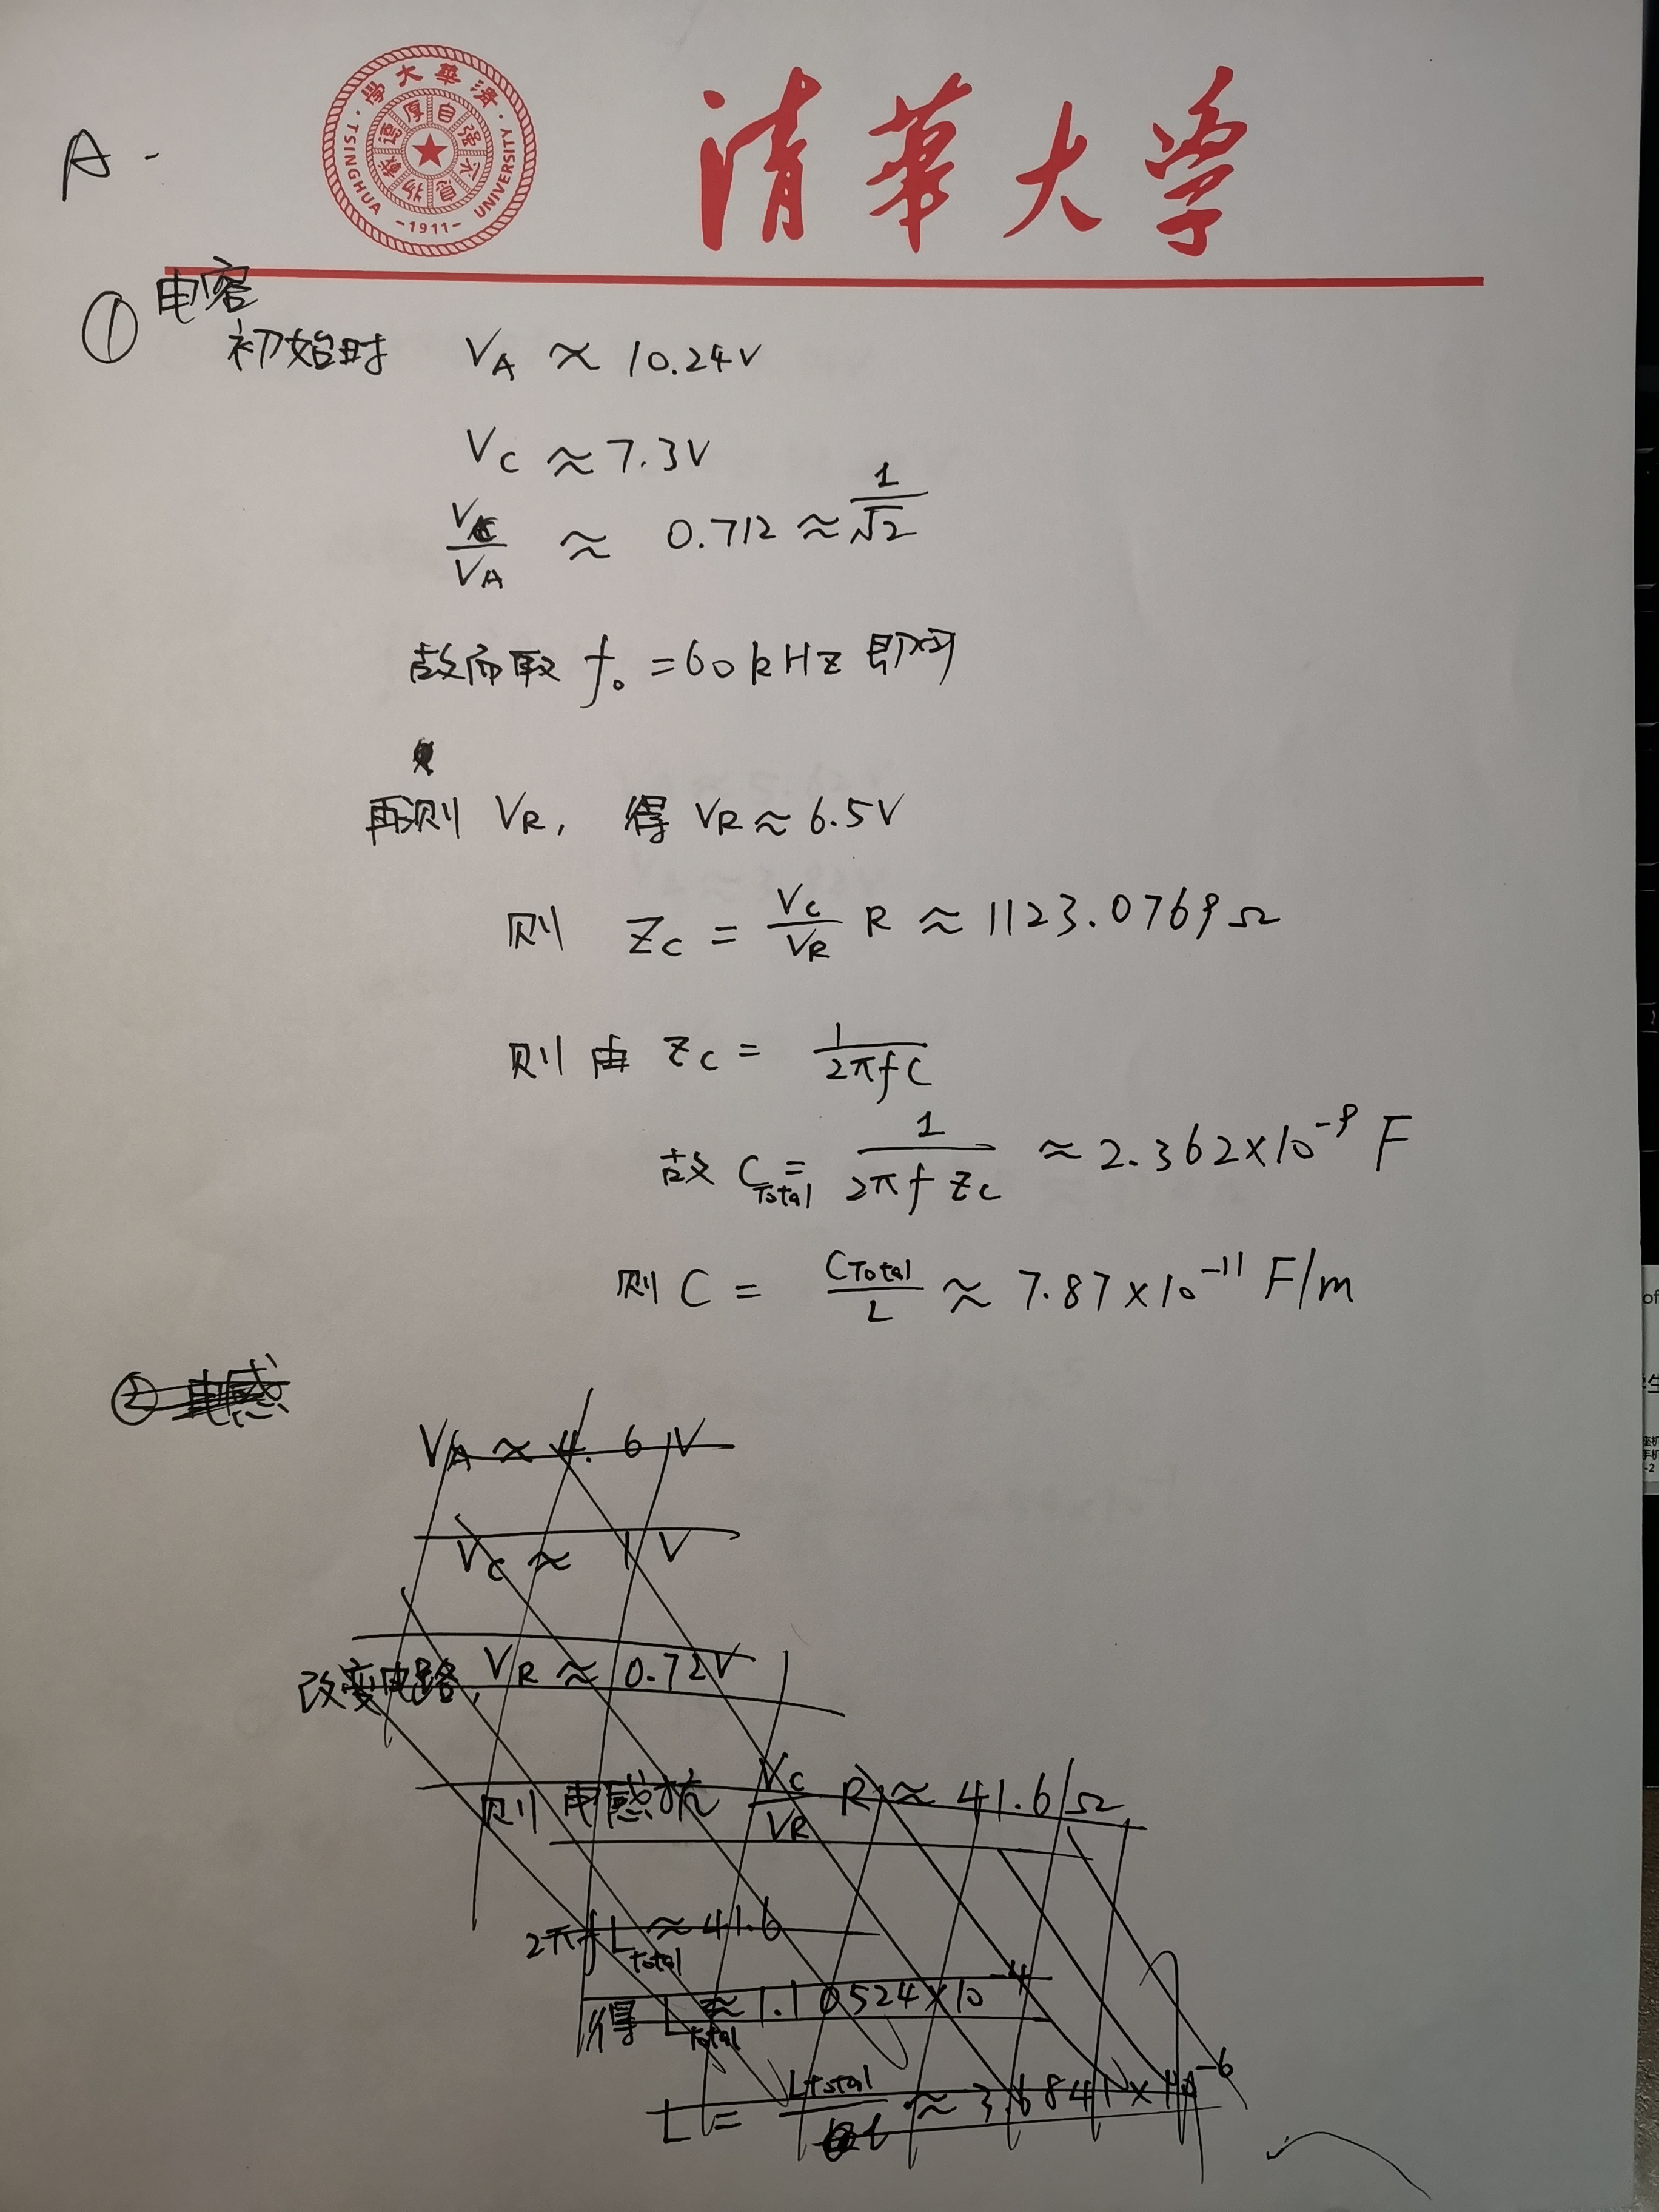
\includegraphics[width=0.95\textwidth]{A1.jpg}
\end{figure}
\begin{figure}[H]
\centering
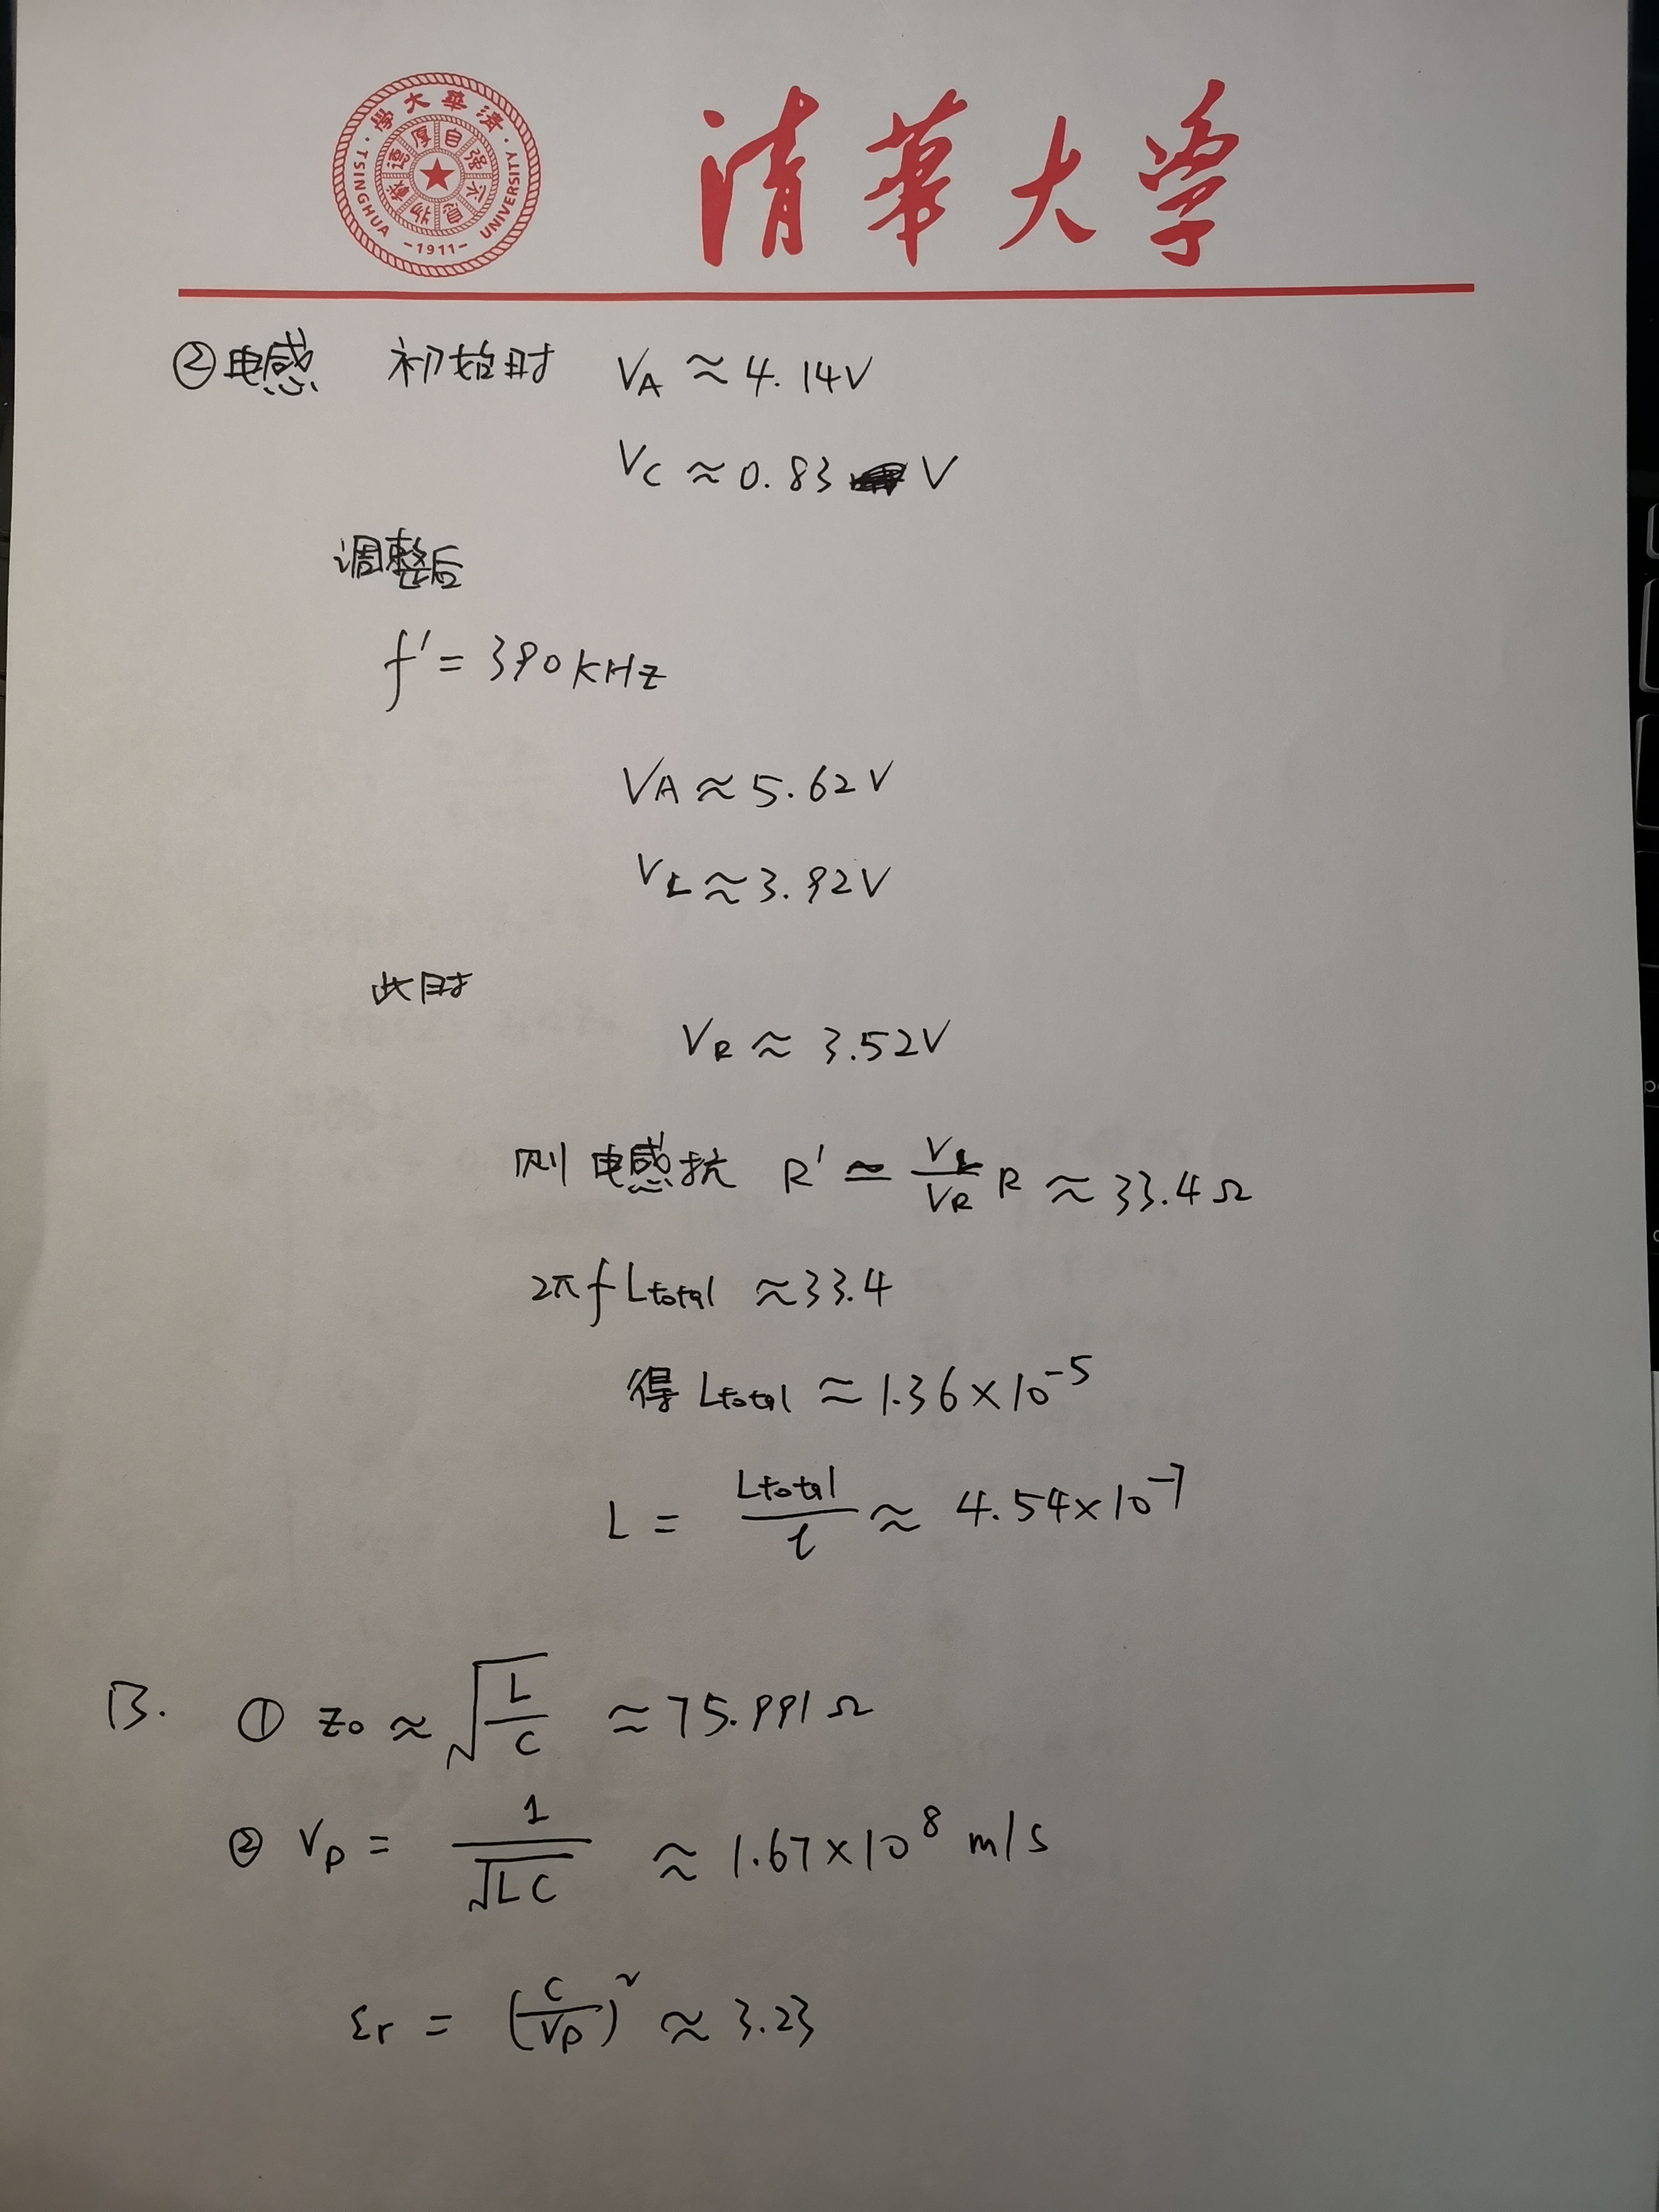
\includegraphics[width=0.95\textwidth]{A2.jpg}
\end{figure}
\begin{figure}[H]
\centering
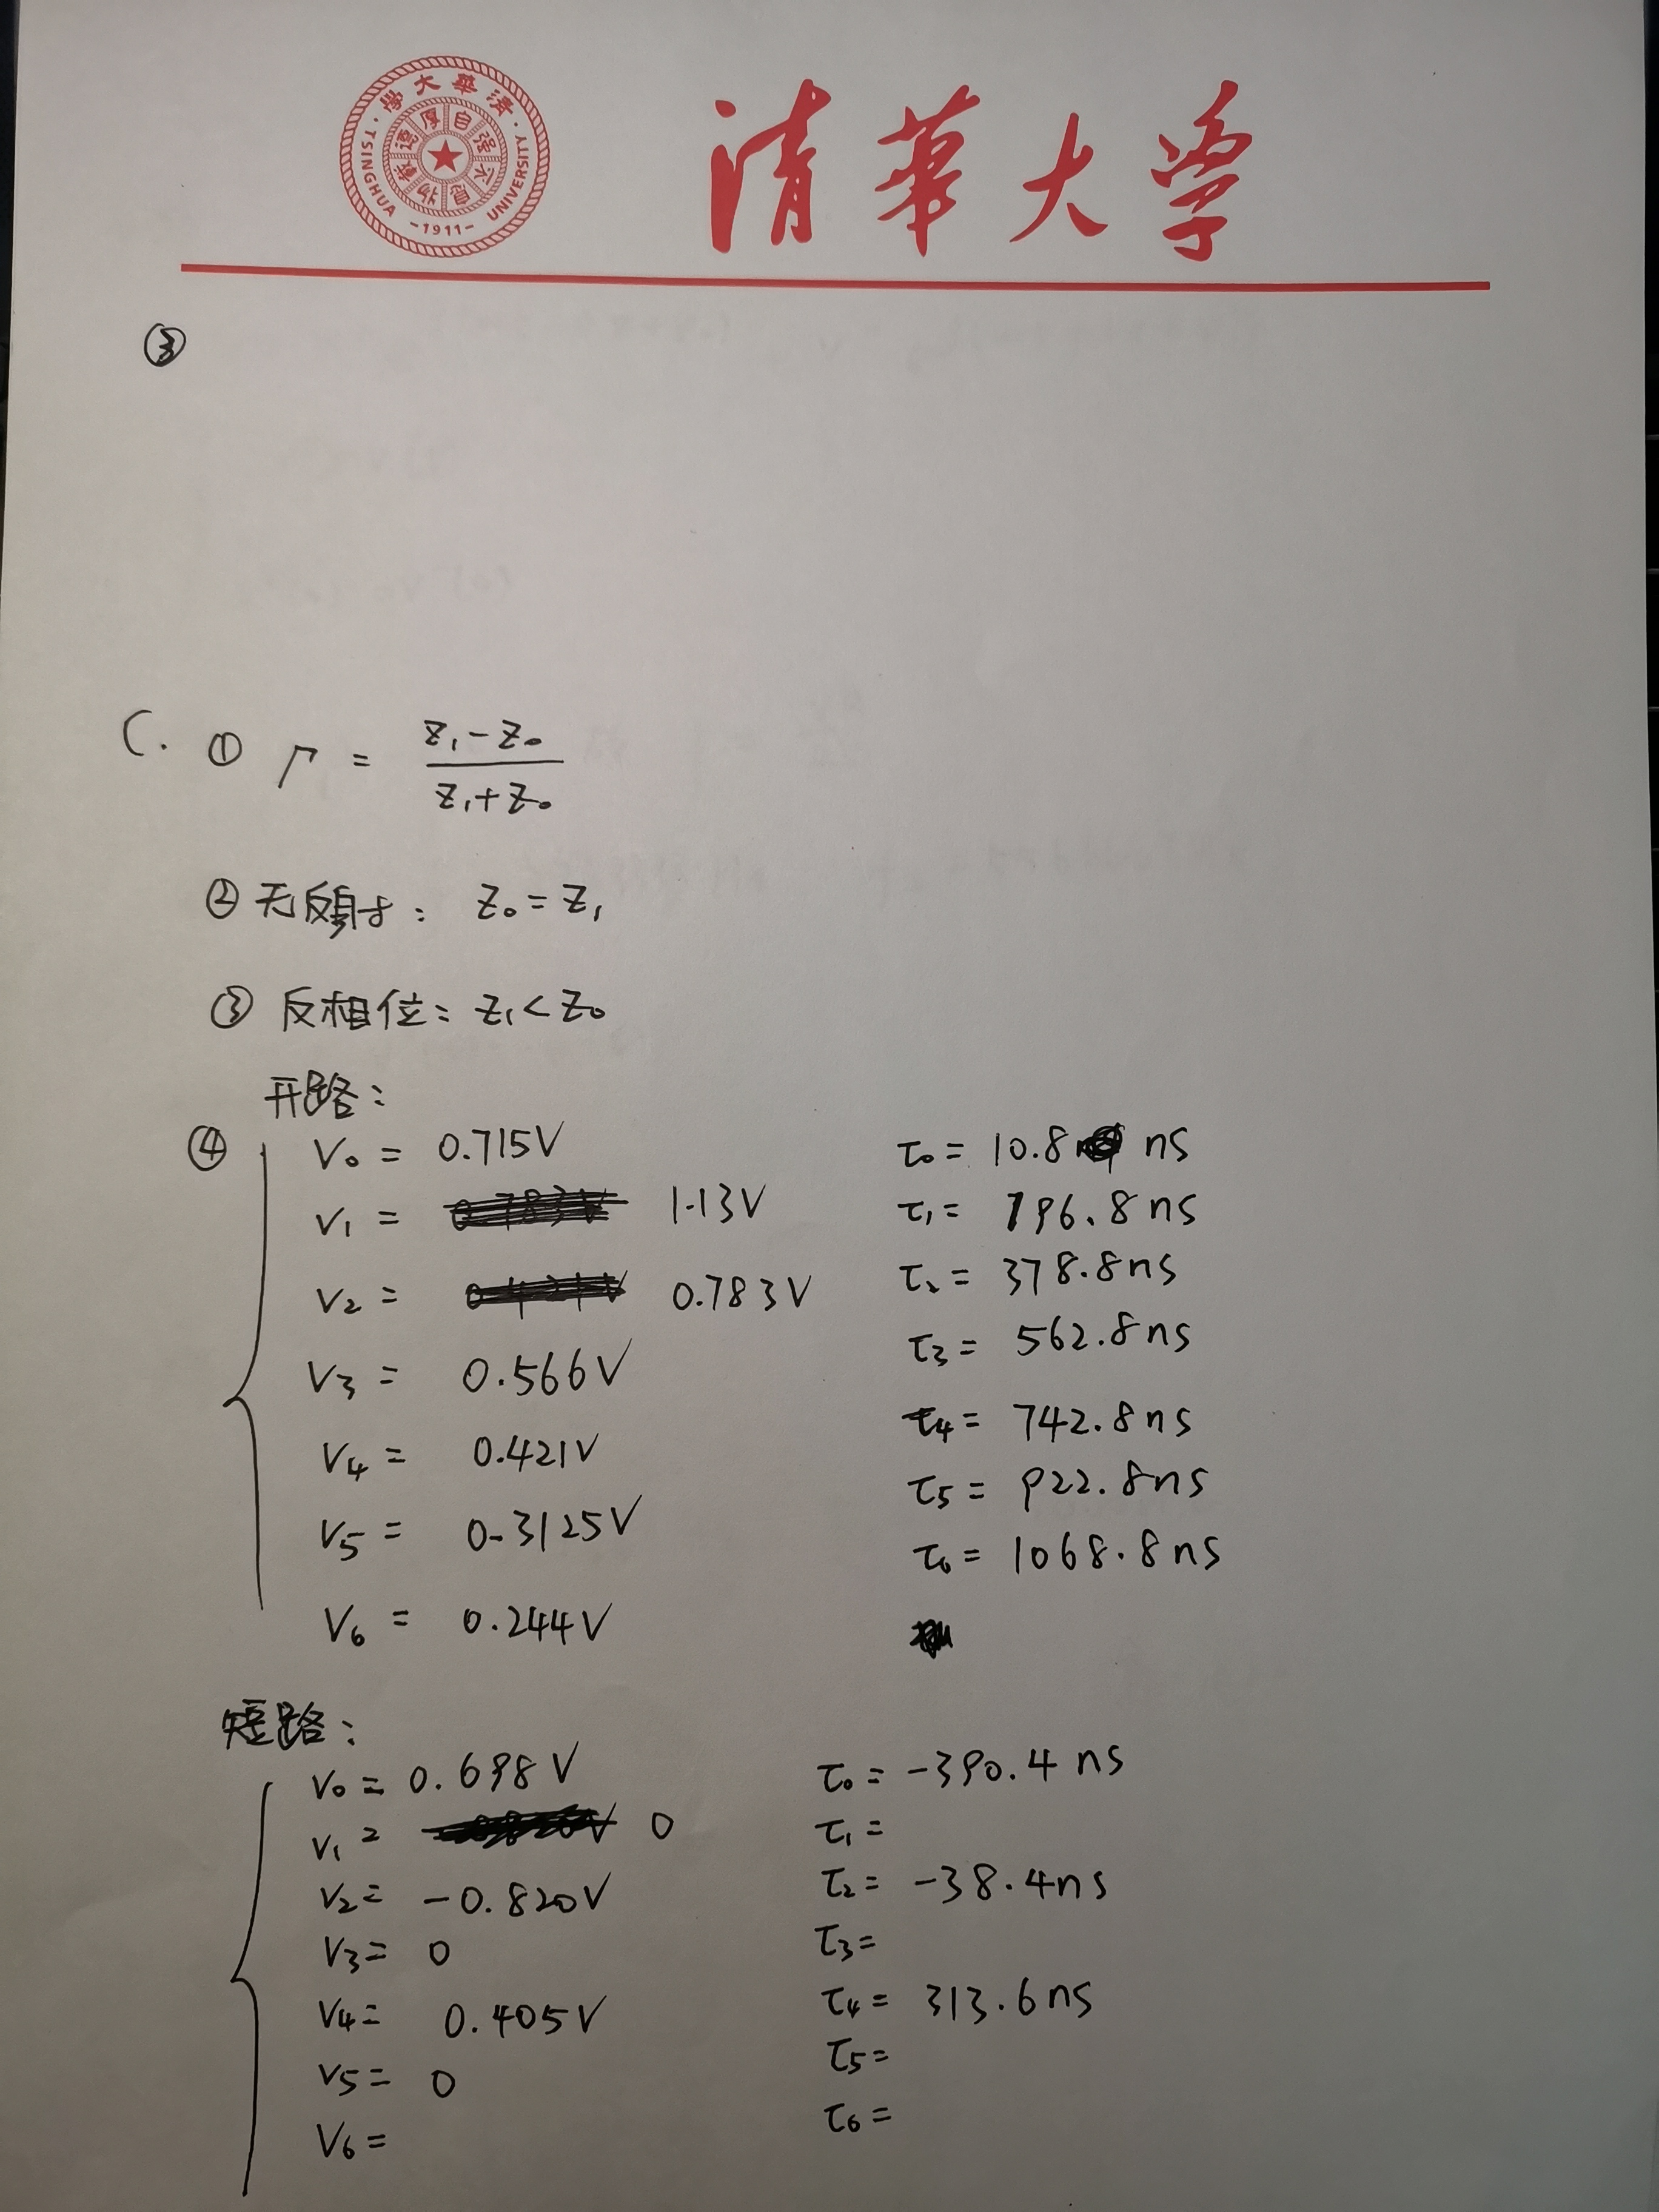
\includegraphics[width=0.95\textwidth]{A3.jpg}
\end{figure}
\begin{figure}[H]
\centering
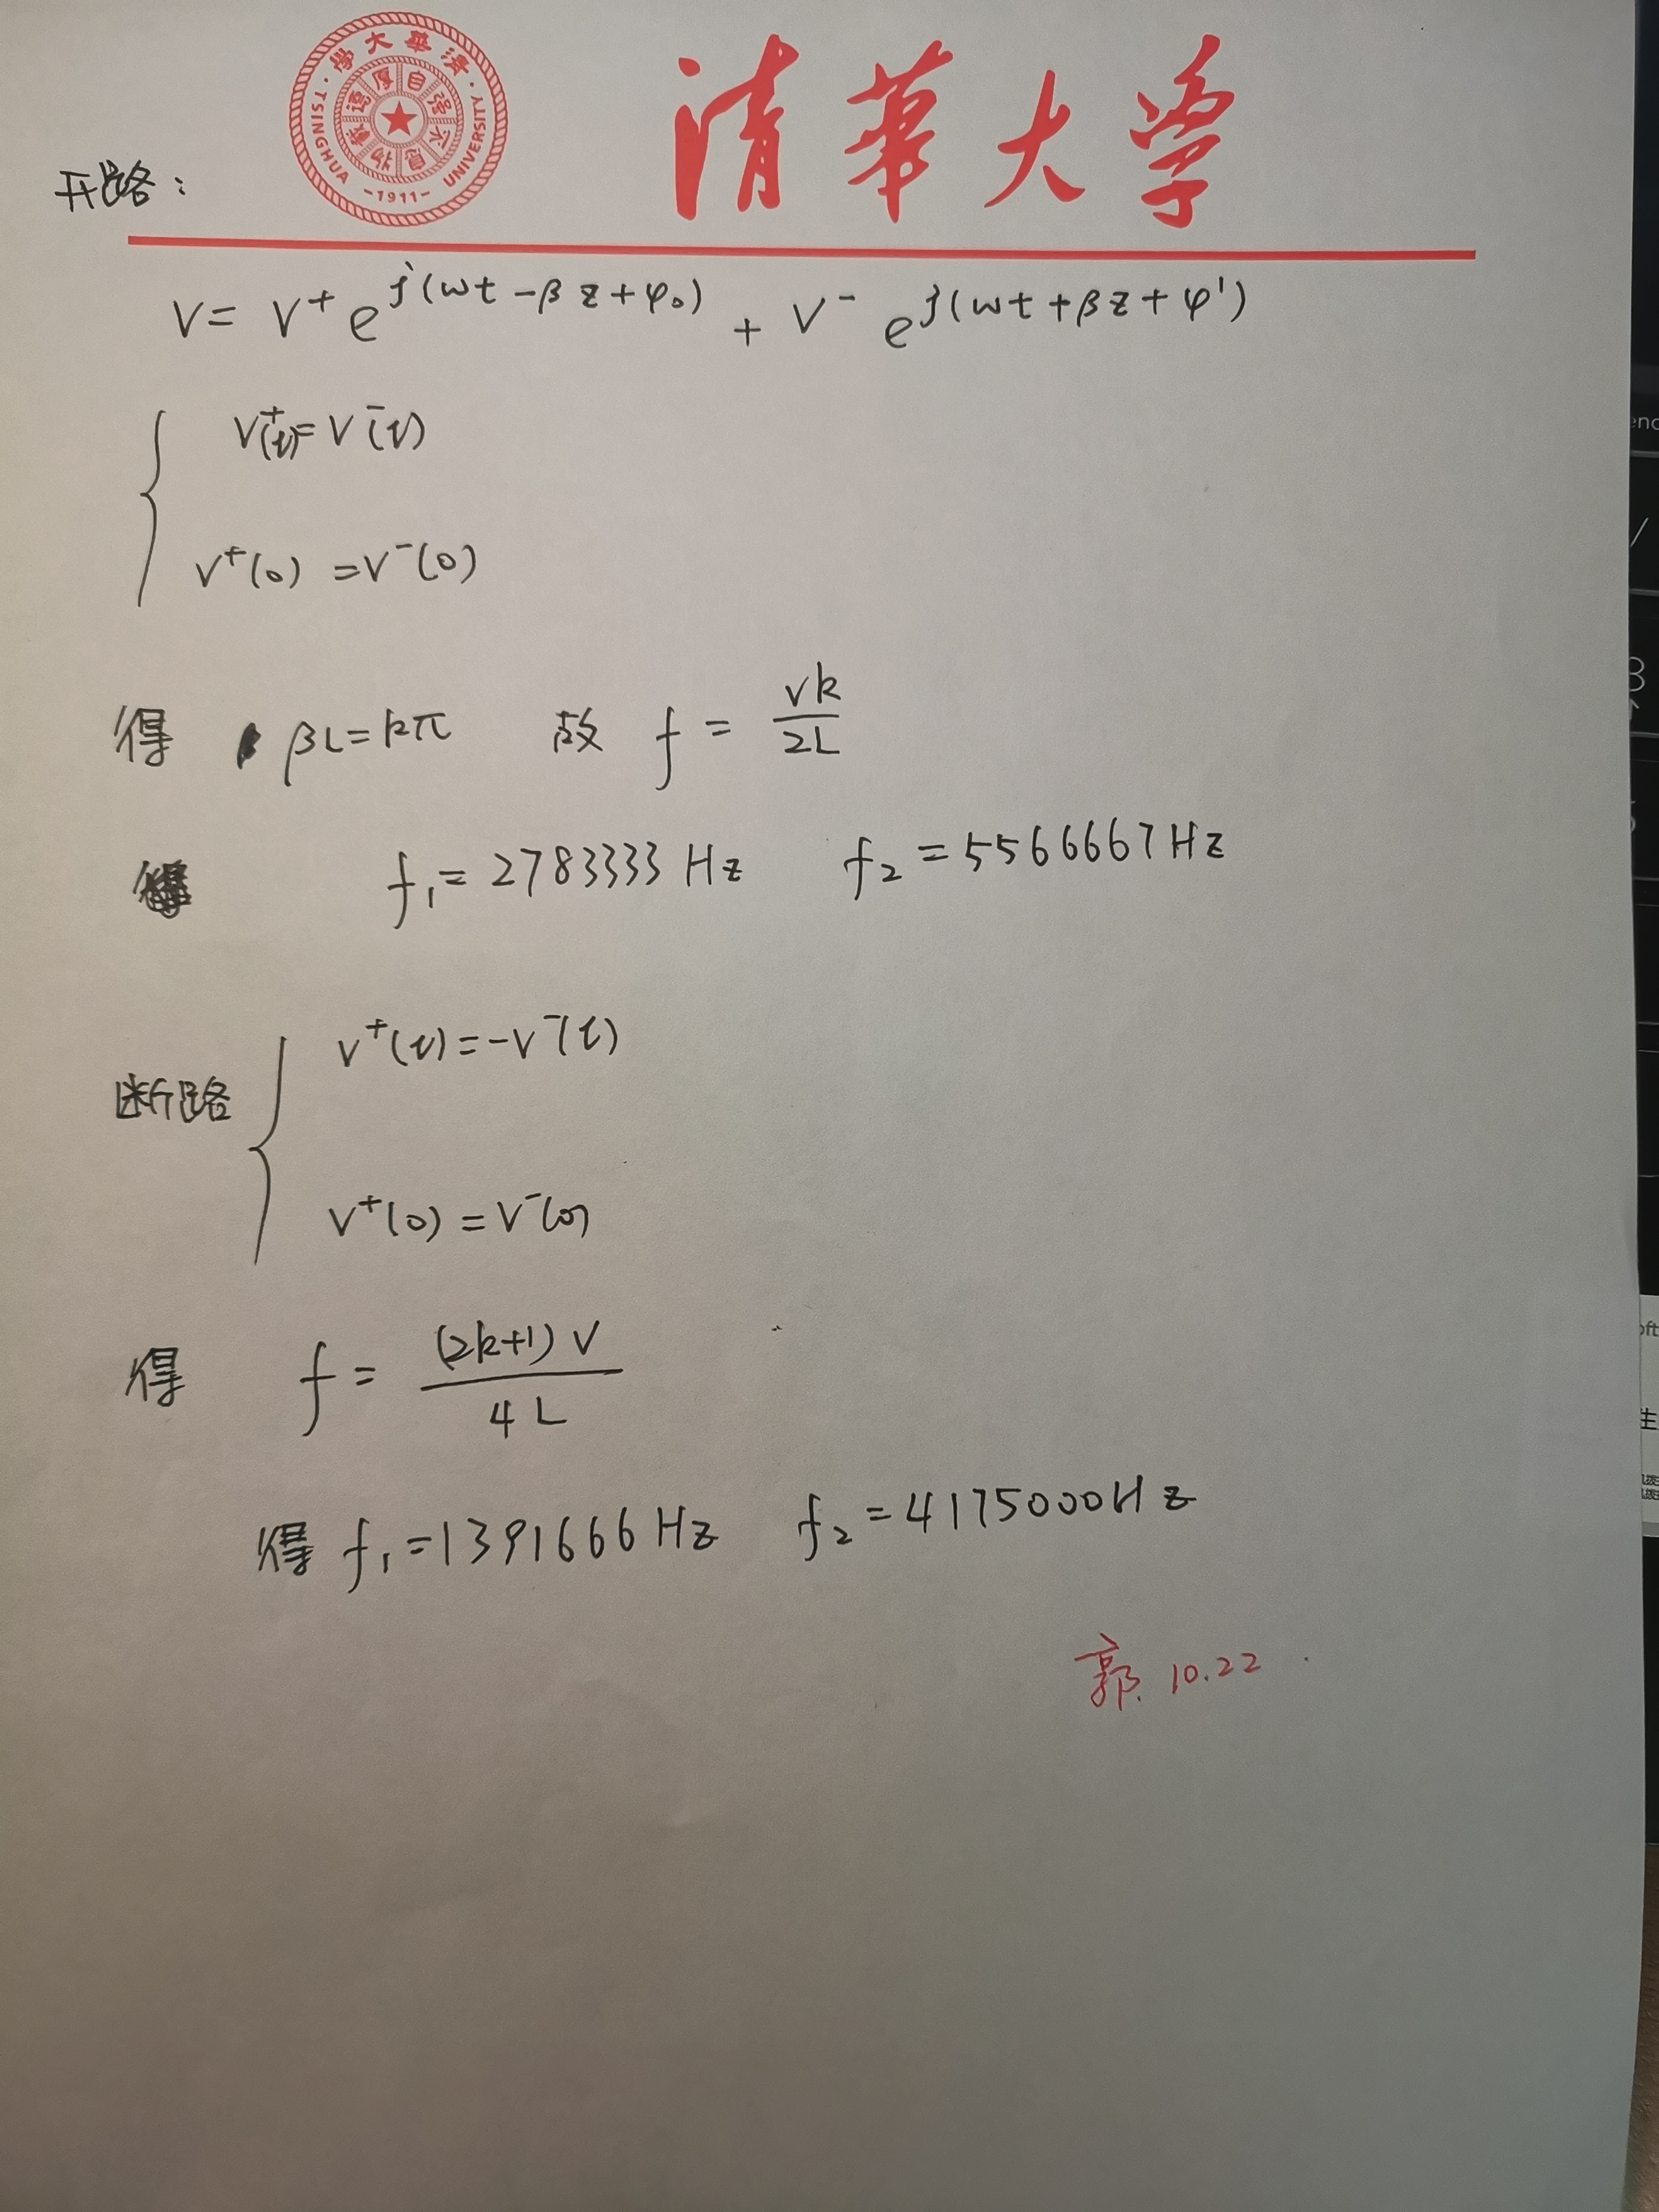
\includegraphics[width=0.95\textwidth]{A4.jpg}
\end{figure}
\begin{thebibliography}{123456} 
\bibitem{ref1}Coaxial cable, Wikipedia
\bibitem{ref2}用于硅基量子计算的自旋读出射频(RF)反射计,2019年亚洲物理奥林匹克竞赛理论题Q1
\bibitem{ref3}Capacitance and inductance of simple transmission lines, Aaron Scher. Oregon Institute of Technology
\bibitem{ref4}数字存储示波器与瞬态信号测量,清华大学物理系物理实验讲义
\bibitem{ref5}微波技术基础。贺瑞霞,陈振国,尹书明,王守平。人民邮电出版社,1988年12月
\bibitem{ref6}Transmission line exercises for the introductory physics laboratory. G.H. Watson. Am. J. Phys., 63(5), pp. 423-425, May 1995
\bibitem{ref7}A wave lab inside a coaxial cable, J. M. Serra, M. C. Brito, J. M. Alves and A. M. Vallera, Eur. J. Phys. 25 (2004) 581–591
\bibitem{ref8}Measuring capacitance \& ESR
\end{thebibliography}


\end{document}
